%==============================================================================
%  Transmission Expansion and Reliability in Peru's Energy Transition:
%  A System Dynamics Approach
%
%  Target journal: Renewable Energy (Elsevier).
%  Class: elsarticle. Build with:  latexmk -pdf main.tex
%
%  Structure: this file carries only the preamble, front matter and the
%  \input list. Each section lives in sections/ so that co-authors can work on
%  one section without colliding in the others.
%==============================================================================
\documentclass[preprint,3p,times,11pt]{elsarticle}

\usepackage[T1]{fontenc}
\usepackage[utf8]{inputenc}
\usepackage{graphicx}
\usepackage{booktabs}
\usepackage{amsmath,amssymb}
\usepackage{siunitx}
\usepackage{multirow}
\usepackage{xcolor}
\usepackage{tikz}
\usetikzlibrary{arrows.meta,positioning,fit,backgrounds,calc,shapes.geometric}
\usepackage[section]{placeins}
\usepackage{subcaption}
\usepackage{url}
\usepackage[hidelinks]{hyperref}

\sisetup{group-separator={,},group-minimum-digits=4,detect-weight=true}
\graphicspath{{figures/}}

% Notes to co-authors. Set \notestrue to show them, \notesfalse before submission.
\newif\ifnotes
\notestrue
\newcommand{\todo}[1]{\ifnotes\textcolor{red}{\textbf{[#1]}}\fi}

% Shorthand for the model's own notation, so a symbol is defined in one place.
\newcommand{\ztech}{\ensuremath{(z,g)}}
\newcommand{\MW}{\si{\mega\watt}}
\newcommand{\GW}{\si{\giga\watt}}
\newcommand{\km}{\si{\kilo\meter}}
\newcommand{\usdmwh}{\si{\USD\per\mega\watt\hour}}
\DeclareSIUnit{\USD}{USD}
\DeclareSIUnit{\month}{month}
\DeclareSIUnit{\year}{yr}
\DeclareSIUnit{\tonne}{t}

\journal{Renewable Energy}

\begin{document}

\begin{frontmatter}

\title{Transmission Expansion and Reliability in Peru's Energy Transition:
       A System Dynamics Approach}

%  \todo{Author list and order to be confirmed by the team before submission.}
\author[eia]{Valentina Betancur}
\author[eia]{Enrique Ángel}
\author[eia]{Mariana Gonzalez}
\author[eia]{Duvan Gomez}
\author[eia]{Carolina Montoya}
\author[eia]{Sebastián Zapata\corref{cor}}
\ead{szapatar@unal.edu.co}
\cortext[cor]{Corresponding author.}
\affiliation[eia]{organization={Universidad EIA},
                  city={Envigado},
                  country={Colombia}}

\begin{abstract}
Peru combines abundant solar, wind and hydro resources with a generation mix still
built on hydropower and natural gas, a longitudinal grid that links three load
zones in series, and a planning process in which generation and transmission
projects advance on very different timescales. Which of these uncertainties
actually governs the system's trajectory is not obvious, and it matters for where
planning effort should go. We build a system dynamics model of the Peruvian power
system, coupled to a congestion-aware dispatch layer, and simulate it monthly from
2025 to 2050 over a designed experiment of 129 runs: a central case, eight
one-at-a-time sensitivity runs, and 120 Latin-hypercube Monte Carlo samples of four
uncertain drivers --- fuel prices, demand growth, and project lead times on the
generation and the transmission side. The result is unambiguous and, we argue,
policy-relevant: demand growth dominates every outcome, with Spearman rank
correlations of 0.99 for transmission length, 0.97 for installed capacity and
$-0.75$ for the average price, while the other three drivers stay below 0.27 in
absolute value. A $\pm$20\,\% band on the 2050 demand level moves required
transmission by $-18.9$\,\% to $+23.8$\,\% and installed capacity by $-24.0$\,\% to
$+29.3$\,\%. The price moves the opposite way to intuition: higher demand lowers
the long-run average price, because it pulls forward low-cost renewable capacity
that the central case defers. Reporting a central, a best and a worst case on a
single declared metric --- the average delivered price --- shows that the
least-cost outcome is also the most transmission-intensive, requiring 26\,\% more
network than the central case. For Peru, the binding planning question is
therefore not how to protect the system against fuel-price risk but whether the
grid can be built fast enough to serve demand that is itself the main source of
uncertainty.
\end{abstract}

\begin{keyword}
Power system expansion planning \sep System dynamics \sep Transmission expansion
\sep Uncertainty analysis \sep Latin hypercube sampling \sep Peru
\end{keyword}

\end{frontmatter}

\section{Introduction}
\label{sec:introduction}

Expansion planning rests on numbers nobody knows. What fuel will cost a decade
out, how fast demand will grow, and how late projects will actually come online
are all uncertain, and each of them is routinely handled by picking a central
value and running a scenario around it. That practice is defensible only if the
uncertainties are of comparable weight. When one of them dominates, effort spent
hedging the others is effort misallocated, and the planning question changes from
\emph{what might happen} to \emph{which unknown is worth managing}.

Peru is a useful place to ask that question, for three reasons. First, the
generation mix is still built on hydropower and natural gas, with non-conventional
renewables at roughly 5\,\% of generation despite a resource base that modelling
work repeatedly finds economically attractive \citep{fiestas2024,delacruz2024}.
Second, the transmission network is longitudinal: three load zones strung in
series along the coast and the Andes, with the best wind and solar resources
systematically distant from the demand they would serve \citep{valdivia2024}.
Third, the institutional record is mixed in an instructive way. The 1992
restructuring produced genuine competition and improved security of supply
\citep{rudnick2019,perezreyes2009}, and Peru was among the regional pioneers of
technology-specific renewable auctions; but the auction mechanism has since been
suspended, leaving developers without a reliable off-take signal, and new
investment in both generation and transmission slowed once the initial wave of
privatisation ran its course. The country therefore holds, simultaneously, a
strong resource endowment, a grid that was not built for it, and a planning
process whose delivery times are themselves uncertain.

Most of the modelling literature addresses this kind of problem with optimisation.
Generation expansion planning, transmission expansion planning and their joint
formulation are mature fields with a large and still-growing body of work
\citep{gacitua2018,babatunde2020,herding2024,tao2025,valipour2026}. These models
are indispensable for identifying what an efficient expansion path would look
like, but they answer a normative question --- what \emph{should} be built ---
under an assumption of perfect rationality and a single optimising agent. The
system they describe is not the system that exists. In a liberalised market,
generation investment is decentralised and driven by expected profitability,
transmission is planned centrally and built on a different and longer clock, and
the gap between the two is bridged by neither \citep{dyner2001,herrera2019}. It is
precisely in that gap that delays, congestion and stranded capacity appear.

System dynamics was developed for exactly this situation: feedback, accumulation
and delay \citep{forrester1997,sterman2000}. Applied to electricity it has a long
record of reproducing the investment cycles, capacity gaps and price swings that
optimisation abstracts away \citep{ford2001,arango2007,assili2008,zapata2018}, and
recent work continues to use it to evaluate policy in liberalised markets
\citep{luo2024,lin2026,oyarzun2026}. What it is less often asked to do is to
quantify, rather than illustrate, the relative weight of the uncertainties that
drive it. A single simulation --- or a handful of named scenarios --- shows what
the model does; it does not show which input the answer actually depends on.

This paper closes that gap for Peru. We build a system dynamics model of the
Peruvian power system, coupled to a congestion-aware dispatch layer, with an
explicit six-stage regulatory and construction pipeline for both generation and
transmission projects. We then subject it to a designed experiment of 129
simulations: a central case, eight one-at-a-time runs that isolate each driver,
and 120 Latin-hypercube Monte Carlo samples in which four drivers move at once ---
fuel prices, demand growth, and project lead times on the generation and on the
transmission side. Every run covers 2025 to 2050 at a monthly step with an hourly
dispatch inside each month.

The contribution is threefold:

\begin{enumerate}
  \item \textbf{A quantified ranking of the uncertainties, not an illustration of
        them.} We report standardised one-at-a-time sensitivities and rank
        correlations over a Latin-hypercube ensemble, together with a convergence
        check on the reported percentiles. The ranking is unambiguous: demand
        growth dominates every indicator we track, and the other three drivers ---
        including fuel prices, the one most often treated as the central risk for a
        gas-dependent system --- are an order of magnitude weaker.
  \item \textbf{A transmission-explicit representation of a longitudinal system.}
        Expansion is disaggregated into grid built for demand, grid built to
        connect new generation, and grid built to interconnect zones, each with its
        own trigger and its own lead time. This matters in Peru because the three
        categories respond to different drivers and only the third is constrained
        by the series topology.
  \item \textbf{A reproducible artefact.} The model, the input workbook, the
        experimental design, the driver, the analysis code and a commented notebook
        that regenerates every figure are openly available. The validation battery,
        the full parameter set and the extended results are given as supplementary
        material.
\end{enumerate}

The central empirical result is counter-intuitive in a way that bears directly on
policy. Higher demand growth does not raise the long-run average price in this
system; it lowers it, because it pulls forward low-cost renewable capacity that
the central case defers. The least-cost trajectory is consequently also the most
transmission-intensive, requiring about a quarter more network than the central
case. For a system whose grid is already the binding constraint, that is not a
comfortable finding, and it reframes the planning problem: the risk to manage in
Peru is not fuel-price exposure but whether transmission can be delivered fast
enough to serve demand growth that is itself the dominant unknown.

The remainder of the paper is organised as follows. Section~\ref{sec:literature}
reviews the relevant literature on transmission planning under energy transition,
infrastructure delays, renewable integration in emerging economies, and system
dynamics in energy planning, and positions the paper against it.
Section~\ref{sec:peru} describes the Peruvian power system.
Section~\ref{sec:methodology} sets out the model, the experimental design and the
validation protocol. Section~\ref{sec:results} reports the central, best and worst
cases and the uncertainty analysis. Section~\ref{sec:discussion} discusses the
implications and Section~\ref{sec:conclusions} concludes.

\section{Literature review}
\label{sec:literature}

\subsection{Transmission planning under the energy transition}
\label{sec:lit:planning}

Transmission is where the energy transition is most visibly constrained. The resources
that decarbonise a system sit where the wind blows and the sun shines, not where load
is concentrated, so every increment of renewable capacity implies an increment of
network --- and the network is planned centrally, built slowly, and remunerated under
rules written for a different fleet.

The modelling response has largely been optimisation. Transmission expansion
planning (TEP) treats a central planner maximising welfare subject to network
constraints, extended steadily to accommodate the transition: stochastic
formulations that make renewable hosting capacity an explicit objective
\citep{valipour2026} and multi-stage investment games for offshore grids
\citep{tao2025}. Joint generation and transmission formulations go further, and the
coordination gain is substantial: \citet{herding2024} find that coordinating the two
reduces total investment by around 10\,\% and network expansion by up to 30\,\%.
Reviews of the field \citep{gacitua2018,babatunde2020} document both its maturity
and its central assumption --- a single rational agent optimising a well-posed
objective.

That assumption is the difficulty here. In a liberalised market the generation investor
and the network planner are different agents acting on different information over
different horizons, and optimisation struggles to represent the structural and
behavioural change policy induces \citep{dyner2001}. \citet{delrio2026} make the point
concretely for Latin America: the cost of capital, not resource quality, determines
which projects are financed.

\subsection{Infrastructure delays and reliability}
\label{sec:lit:delays}

A transmission project that is planned but late is, for the duration of the delay,
indistinguishable from one that was never planned. \citet{ritter2019} simulate
delayed interconnector expansion in a high-renewable European system and show the
delay does not merely postpone benefits: it raises emissions and generation costs,
because surplus renewable energy that cannot be moved is replaced by conventional
generation elsewhere, altering the final mix. \citet{herrera2019} reach a
structurally similar conclusion for northeast Brazil, where transmission constraints
bound wind expansion directly. The mechanism is the same in both: generation
investment responds to a connection opportunity the network has not yet delivered.

The causes of delay are largely non-technical. Right-of-way disputes, licensing and
local opposition recur across jurisdictions; \citet{sun2026} quantify the last of
these, and \citet{boateng2026} generalise the point, identifying
institutional-quality thresholds below which renewable deployment responds very
differently to identical incentives. For a system such as Peru's, lead-time risk is
therefore better modelled as an institutional variable than an engineering one.

\subsection{Renewable integration in emerging economies}
\label{sec:lit:emerging}

Emerging economies face the integration problem with more expensive capital, thinner
institutions, and grids that are radial or longitudinal rather than meshed.
\citet{dasilva2025} find the regional efficiency of Brazilian renewable expansion
varying sharply by region, consistent with network access rather than resource quality
being the differentiator, while \citet{antoniolli2022}, \citet{wu2025} and
\citet{sheng2026} document rooftop and community-scale generation as mechanisms that
reduce the inter-zonal transfers a longitudinal grid must support.

The alternative to building network is using it harder. Grid-enhancing technologies
raise transfer capability without new right-of-way --- \citet{sadeghian2026} formalise
dynamic thermal line rating under chance constraints --- though remuneration
frameworks for them are generally absent. Storage plays the complementary role:
\citet{sousa2024} quantify the substitution between storage and other flexibility
resources, making the structural point that the transmission a system needs is not
independent of how much flexibility it builds.

\subsection{System dynamics in energy planning}
\label{sec:lit:sd}

System dynamics takes the opposite stance: rather than solving for the best
configuration, it simulates the configuration the system's own feedback, accumulation
and delay will produce \citep{forrester1997,sterman2000}. For electricity this is
productive because the pathologies of interest --- investment cycles, capacity gaps,
price spikes following construction lags --- are consequences of structure rather than
of optimisation failure.

The lineage is long: \citet{ford2001} explained the California capacity crisis as a
construction-delay phenomenon, \citet{arango2007} simulated alternative regulation in
Colombia, \citet{assili2008} examined capacity payments with construction delays
explicit, and \citet{simshauser2010} connected resource adequacy to investment
uncertainty. Recent work extends this to transition pathways
\citep{zapata2018,morcillo2018,luo2024}, carbon border adjustment \citep{lin2026} and
PV adoption policy \citep{oyarzun2026}.

Model confidence in system dynamics is established by a documented battery of tests
rather than a goodness-of-fit statistic \citep{barlas1996,oliva2004}, and recent
methodological work reconsiders what confidence means for models used exploratorily
rather than predictively \citep{richardson2024}. We follow that protocol explicitly
and report it in full in the supplementary material.

Where this literature is thinnest is uncertainty quantification. Scenario analysis is
near-universal; designed sampling of the input space is rare. The tools are standard
outside system dynamics --- Latin hypercube sampling \citep{mckay1992} and
regression- or variance-based global sensitivity measures \citep{homma1996} --- and
are used in power system work, for instance in \citeauthor{alvarez2026}'s
\citeyearpar{alvarez2026} probabilistic assessment of the Spanish 2030 system.
Combining them with a feedback-rich simulation model is the step this paper takes.

\subsection{Peruvian and Latin American studies, and the gap}
\label{sec:lit:gap}

Peru's restructuring is studied as a reference case: a reform that delivered
competition and improved security of supply while accumulating a high reserve margin
and fossil dependence \citep{rudnick2019,perezreyes2009}. Recent work addresses the
transition itself \citep{fiestas2024,delacruz2024} and the network
\citep{valdivia2024}. Regionally, \citet{sauma2006} established the
proactive-versus-reactive distinction in transmission valuation, while analyses of
Andean interconnection identify regulatory sovereignty rather than transfer capability
as the barrier \citep{guliev2022,sempertegui2017}.

Three gaps follow. First, the delay literature establishes that lead times matter but
not how much, relative to other uncertainties, in a common design. Second, the system
dynamics energy literature rarely quantifies uncertainty with a designed experiment,
so a small number of named scenarios cannot separate a structural result from an
artefact of one input assumption. Third, Peru is under-represented: existing studies
are either optimisation-based assessments of a renewable target
\citep{fiestas2024,delacruz2024} or operational analyses of the network
\citep{valdivia2024}, and none represents the investment-and-delay feedback between
generation and transmission that a longitudinal, gas-dependent system with suspended
auctions would be expected to exhibit. This paper addresses all three.

\section{The Peruvian power system}
\label{sec:peru}

\subsection{Market structure and generation mix}
\label{sec:peru:overview}

Following a macroeconomic collapse in the late 1980s, Peru moved from an integrated
state system to a competitive wholesale market with marginal nodal prices, capacity
payments and bilateral contracts. The Electric Concessions Law of 1992 unbundled
generation, transmission and distribution, and the supply auctions introduced from
2006 consolidated productivity gains, with clear efficiency improvements in
distribution after restructuring \citep{rudnick2019,perezreyes2009}.

The generation matrix remains dominated by hydropower and natural gas. By 2015 the
mix was roughly 50\,\% hydro and 45\,\% gas, with thermal sources overall accounting
for about 41\,\% of generation by 2017 \citep{rudnick2019}. The dependence is
structural: over half the natural gas consumed in the country goes to power plants
\citep{enerdata2024}, making electricity the primary driver of gas demand and
exposing it to price and supply shocks. Despite substantial solar, wind, geothermal
and biomass potential, non-conventional renewables supplied only about 5\,\% of
generation by 2022 \citep{campodonico2022}.

\citet{fiestas2024} find that raising non-conventional renewables to 28\,\% of the
matrix would cut gas consumption by \SI{2.04}{\kilo\meter\cubed} and avoid
\SI{4.99}{\mega\tonne} CO$_2$-eq annually while reducing system costs, and
\citet{delacruz2024} reach compatible conclusions to 2050. The economic case is
established; the route is not. The auction mechanism that for a decade channelled
renewable investment has been suspended, leaving developers without a reliable off-take
signal \citep{campodonico2022,torres2026}, and the grid was not built with variable
renewables in mind. This combination is not unusual: institutional quality and the cost
of capital, rather than resource quality, condition deployment
\citep{boateng2026,delrio2026}.

\subsection{Zonal structure and transmission}
\label{sec:peru:zones}

The model represents the system as three zones connected in series
(Figure~\ref{fig:map}). This is not a simplification for tractability but the
physical topology: Peru's main grid runs longitudinally, so the southern zone
reaches the rest of the system only through the centre. Table~\ref{tab:zones}
reports the January 2025 starting condition. The centre zone holds 60\,\% of
installed capacity; the Z1--Z2 and Z2--Z3 corridors provide \SI{900}{\mega\watt} and
\SI{700}{\mega\watt} of transfer capability; there is no direct Z1--Z3 path. A
series topology has no redundancy: a constraint on the central corridor isolates a
third of the system, and every transfer between the extremes consumes capacity on
both corridors.

\begin{figure}[tb]
  \centering
  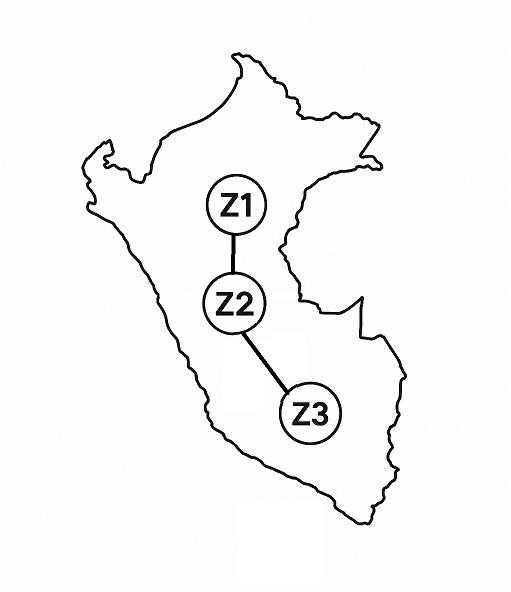
\includegraphics[width=0.40\textwidth]{mapa.png}
  \caption{Zonal representation of the Peruvian power system: north (Z1), centre
  (Z2) and south (Z3) in series. All exchange between the extremes transits the
  centre.}
  \label{fig:map}
\end{figure}

\begin{table}[tb]
  \centering
  \caption{Initial condition, January 2025, as represented in the model. Technology
  shares are given in Supplementary Material~S2.}
  \label{tab:zones}
  \small
  \begin{tabular}{@{}llrr@{}}
    \toprule
    Zone & Description & Capacity [\si{\mega\watt}] & Share \\
    \midrule
    Z1 & North   & \num{1606.1} & 11.4\,\% \\
    Z2 & Centre  & \num{8461.9} & 60.2\,\% \\
    Z3 & South   & \num{3989.0} & 28.4\,\% \\
    \midrule
    \multicolumn{2}{@{}l}{\textbf{Total}} & \textbf{\num{14057.0}} & 100\,\% \\
    \midrule
    \multicolumn{4}{@{}l}{\emph{Corridors:} Z1--Z2 \SI{900}{\mega\watt} over
      \SI{232.3}{\kilo\meter}; Z2--Z3 \SI{700}{\mega\watt} over \SI{271.8}{\kilo\meter}} \\
    \multicolumn{4}{@{}l}{\emph{Network:} \SI{16180}{\kilo\meter} total;
      thermal and reservoir hydro are 78\,\% of capacity, wind and solar 10.7\,\%} \\
    \bottomrule
  \end{tabular}
\end{table}

Congestion management in Peruvian planning has become more sophisticated, with
$n-1$ contingency screening alongside demand, generation, fuel-price and weather
projections \citep{valdivia2024}. At regional level, Andean interconnection is
technically and economically feasible but has stalled on regulatory sovereignty
rather than engineering \citep{sempertegui2017,guliev2022}.

\subsection{Planning challenges and the modelling implication}
\label{sec:peru:delays}

The gains from the 1990s reform were real but uneven. Once the initial wave of
privatisation ran its course, investment in generation and transmission slowed
considerably, indicating that the regulatory framework was not generating the
long-term certainty infrastructure capital requires \citep{rudnick2019}. The
suspension of the auction mechanism has hit onshore wind hardest: projects conceived
for structured procurement now compete in a spot market under price uncertainty,
and the best wind resources remain far from consumption \citep{torres2026}. Fossil
dependence and a renewable share of roughly 5.5\,\% of total energy leave Peru
exposed to external price swings \citep{colinacalvo2024}.

This is the feature that motivates the modelling choice in
Section~\ref{sec:methodology}. Lead times here are an institutional outcome rather
than an engineering parameter, and they differ systematically between generation,
which responds to a market signal, and transmission, which is planned centrally and
delivered on a longer clock. Representing that asymmetry explicitly is what allows
the model to be asked which of the two binds.

Peru is instructive comparatively: simultaneously a reference case for successful
market reform and a cautionary example of its limits --- competition and improved
security of supply, but increasing fossil dependence and a high reserve margin
\citep{rudnick2019}; early leadership in renewable auctions, but no consolidated
transition strategy, a gap visible against Chile, which started from a comparable base
and has moved further \citep{reyes2025,guliev2022}.

\section{Methodology}
\label{sec:methodology}

\subsection{Approach}
\label{sec:method:approach}

The question requires two things usually provided separately: a model whose behaviour
arises from the structure of the decision process rather than from an optimality
assumption, because the phenomenon of interest is the mismatch between a decentralised
generation market and a centrally planned network; and a designed experiment over the
inputs, because a ranking cannot be read off a handful of named scenarios.

We therefore combine a system dynamics model with a Latin-hypercube designed
experiment. The simulation runs monthly from January 2025 to January 2050 (300 months,
integration step \SI{0.25}{\month}), with an hourly dispatch represented inside each
month by one representative day of 24 hourly levels. The experiment comprises 129 runs:
one central case, two one-at-a-time runs per factor, and 120 Monte Carlo samples in
which all four factors vary simultaneously. One-at-a-time runs isolate each factor
against a fixed reference, which makes a tornado bar attributable but says nothing
about interaction; the Monte Carlo ensemble moves everything at once, which the
percentile envelopes and rank correlations require but leaves individual effects to be
inferred statistically. Reporting both, and checking they agree, is stronger than
either alone.

\subsection{Model structure}
\label{sec:method:structure}

Figure~\ref{fig:model} shows the modules, flows and governing parameters. The full
equation set is in Supplementary Material~S1 and the complete parameter set, with the
workbook cell of every value, in Supplementary Material~S2.

% Block diagram of the model: modules, the flows between them, and the parameters
% that govern each one. The four sensitivity knobs of the experiment are drawn in
% the accent colour so the reader can see where in the structure they act.
%
% Laid out on an explicit coordinate grid rather than with relative positioning:
% the boxes carry enough text that `below=of` chains drift and overlap. Outputs sit
% in a bottom row rather than a right-hand column, which is what keeps the figure
% inside the text width.
\begin{figure*}[tb]
\centering
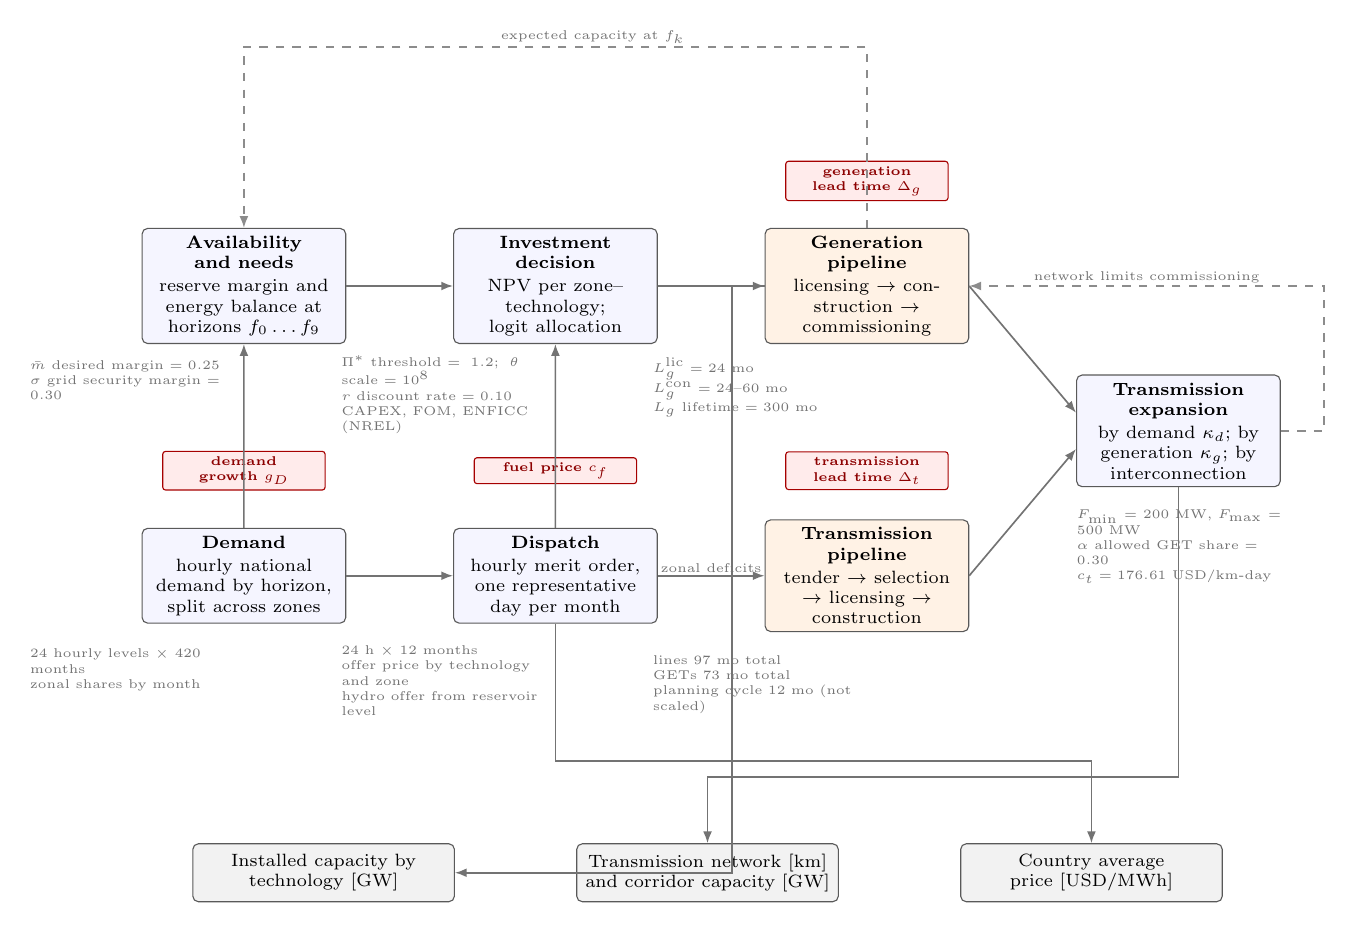
\begin{tikzpicture}[
  x=1cm, y=1cm, scale=0.92, transform shape,
  mod/.style={draw=black!65, rounded corners=2pt, fill=blue!4, align=center,
              text width=26mm, minimum height=13mm, inner sep=3pt, font=\scriptsize},
  pipe/.style={mod, fill=orange!10},
  outp/.style={draw=black!65, rounded corners=2pt, fill=black!5, align=center,
               text width=34mm, minimum height=8mm, inner sep=3pt, font=\scriptsize},
  par/.style={align=left, font=\tiny, text=black!55, text width=29mm, inner sep=1pt},
  knob/.style={draw=red!65!black, fill=red!8, rounded corners=1pt, align=center,
               font=\tiny\bfseries, inner sep=2pt, text=red!55!black, text width=21mm},
  fl/.style={-{Latex[length=1.5mm]}, draw=black!55, semithick},
  fb/.style={-{Latex[length=1.5mm]}, draw=black!45, semithick, dashed},
  lbl/.style={font=\tiny, text=black!55, inner sep=1pt},
]

\def\rA{7.2}   % top row: needs, decision, generation pipeline
\def\rB{3.2}   % bottom row: demand, dispatch, transmission pipeline
\def\rM{5.2}   % transmission expansion, between the two rows
\def\rO{-0.9}  % outputs

% ============ column 1 ======================================================
\node[mod]  (need) at (0,\rA) {\textbf{Availability and needs}\\[1pt]
  reserve margin and energy balance at horizons $f_0 \dots f_9$};
\node[par]  at (-1.5,\rA-1.3) {$\bar m$ desired margin $=0.25$\\
                               $\sigma$ grid security margin $=0.30$};

\node[mod]  (dem) at (0,\rB) {\textbf{Demand}\\[1pt]
  hourly national demand by horizon, split across zones};
\node[par]  at (-1.5,\rB-1.3) {24 hourly levels $\times$ 420 months\\
                               zonal shares by month};
\node[knob] (kdem) at (0,\rB+1.45) {demand growth $g_D$};

% ============ column 2 ======================================================
\node[mod]  (inv) at (4.3,\rA) {\textbf{Investment decision}\\[1pt]
  NPV per zone--technology; logit allocation};
\node[par]  at (2.8,\rA-1.5) {$\Pi^{*}$ threshold $=1.2$;\;
                              $\theta$ scale $=10^{8}$\\
                              $r$ discount rate $=0.10$\\
                              CAPEX, FOM, ENFICC (NREL)};

\node[mod]  (disp) at (4.3,\rB) {\textbf{Dispatch}\\[1pt]
  hourly merit order, one representative day per month};
\node[par]  at (2.8,\rB-1.45) {24 h $\times$ 12 months\\
                               offer price by technology and zone\\
                               hydro offer from reservoir level};
\node[knob] (kfuel) at (4.3,\rB+1.45) {fuel price $c_f$};

% ============ column 3 ======================================================
\node[pipe] (gpipe) at (8.6,\rA) {\textbf{Generation pipeline}\\[1pt]
  licensing $\to$ construction $\to$ commissioning};
\node[par]  at (7.1,\rA-1.4) {$L^{\text{lic}}_{g}=24$ mo\\
                              $L^{\text{con}}_{g}=24$--60 mo\\
                              $L_{g}$ lifetime $=300$ mo};
\node[knob] (kgen) at (8.6,\rA+1.45) {generation lead time $\Delta_g$};

\node[pipe] (tpipe) at (8.6,\rB) {\textbf{Transmission pipeline}\\[1pt]
  tender $\to$ selection $\to$ licensing $\to$ construction};
\node[par]  at (7.1,\rB-1.5) {lines $97$ mo total\\
                              GETs $73$ mo total\\
                              planning cycle $12$ mo (not scaled)};
\node[knob] (ktr) at (8.6,\rB+1.45) {transmission lead time $\Delta_t$};

% ============ column 4 ======================================================
\node[mod]  (tcat) at (12.9,\rM) {\textbf{Transmission expansion}\\[1pt]
  by demand $\kappa_d$; by generation $\kappa_g$; by interconnection};
\node[par]  at (12.95,\rM-1.6) {$F_{\min}=200$ MW, $F_{\max}=500$ MW\\
                                $\alpha$ allowed GET share $=0.30$\\
                                $c_t=176.61$ USD/km-day};

% ============ outputs (bottom row) =========================================
\node[outp] (out1) at (1.1,\rO)  {Installed capacity by technology [GW]};
\node[outp] (out2) at (6.4,\rO)  {Transmission network [km] and corridor capacity [GW]};
\node[outp] (out3) at (11.7,\rO) {Country average price [USD/MWh]};

% ============ flows ========================================================
\draw[fl] (dem)        -- (need);
\draw[fl] (need)       -- (inv);
\draw[fl] (dem.east)   -- (disp.west);
\draw[fl] (disp)       -- (inv);
\draw[fl] (inv)        -- (gpipe);
\draw[fl] (disp.east)  -- node[lbl, above] {zonal deficits} (tpipe.west);
\draw[fl] (gpipe.east) -- ([yshift=2.5mm]tcat.west);
\draw[fl] (tpipe.east) -- ([yshift=-2.5mm]tcat.west);

\draw[fl] (gpipe.west) -- ++(-0.45,0) |- (out1.east);
\draw[fl] (tcat.south) -- ++(0,-4.0) -| (out2.north);
\draw[fl] (disp.south) -- ++(0,-1.9) -| (out3.north);

% ============ the two feedbacks ============================================
\draw[fb] (tcat.east) -- ++(0.6,0) |- node[lbl, pos=0.75, above]
  {network limits commissioning} (gpipe.east);
\draw[fb] (gpipe.north) -- ++(0,2.5) -| node[lbl, pos=0.22, above]
  {expected capacity at $f_k$} (need.north);

\end{tikzpicture}
\caption{Structure of the model. Solid arrows are material and information flows
within a simulation step; dashed arrows are the two feedbacks that generate the
behaviour of interest --- commissioning is constrained by the network that has
actually been delivered, and investment decisions are taken on expected rather than
current capacity. Grey text gives the governing parameters and their central
values; the four boxes in red are the uncertain drivers varied in the designed
experiment of Section~\ref{sec:method:design}.}
\label{fig:model}
\end{figure*}


\subsubsection{Generation: investment, pipeline, commissioning}
\label{sec:method:gen}

Generation capacity is a stock fed by a pipeline in which committed projects pass
through licensing and construction before commissioning, with total lead time
$(L^{\text{lic}}_{z,g} + L^{\text{con}}_{z,g})(1+\Delta_g)$ --- licensing at 24 months
for every technology, construction from 24 months (PV) to 60 (reservoir hydro).
Commissioning is bounded by the network actually delivered: capacity that has finished
construction cannot enter until there is transmission to evacuate it. This is the first
of the two feedbacks drawn dashed in Figure~\ref{fig:model}, and it is what couples the
generation market to the network plan.

Investment is triggered two ways. Under adequacy, a shortfall of the expected reserve
margin below the desired margin $\bar m$ becomes a capacity requirement. Under
profitability, the model computes a net present value per zone--technology over a
25-year life --- assuming the plant is the only entrant and that current plus committed
capacity persists, with CAPEX, fixed O\&M, fuel and firm-capacity parameters from
\citet{nrel2024} --- admits options above a threshold $\Pi^{*}$, and allocates them
across technologies by a logit share with scale $\theta$. That share represents the
dispersion of investor beliefs rather than a single optimising agent, and is the point
at which the model departs most clearly from a GEP formulation. Decisions use
\emph{expected} rather than current state: expected capacity at 3, 5, 7 and 9 years
includes the pipeline, so investors know the construction times they face. This second
feedback prevents over-investment against a deficit already being remedied.

\subsubsection{Transmission: three categories, three triggers}
\label{sec:method:trans}

Transmission expansion is disaggregated because the categories respond to different
drivers and carry different lead times. Network \emph{for demand} follows zonal peak
growth at an empirical intensity $\kappa_d$ and carries no construction delay, since
the model does not represent intra-zonal networks. Network \emph{for generation}
connects each new plant at intensity $\kappa_g$, triggered by the formal identification
of a project at a planning horizon --- structurally \emph{reactive}, responding to
confirmed rather than anticipated projects, which combined with transmission lead times
exceeding generation lead times is a principal source of the bottleneck studied here.
Network \emph{for interconnection} is triggered when a transfer implied by the dispatch
exceeds delivered corridor capability, met by a grid-enhancing technology if the
shortfall is at most a share $\alpha$ of current capability and by a new line
otherwise, with increments bounded by $F_{\min}$ and $F_{\max}$ to represent lumpiness.

Transmission projects pass a four-stage pipeline --- tender, investor selection,
licensing, construction --- totalling 97 months for lines and 73 for GETs, each stage
scaled by $(1+\Delta_t)$. The 12-month planning cycle is deliberately not scaled: the
model uses it as the period of a modulo operation setting when plans are revised.

\subsubsection{Dispatch, prices and distributed resources}
\label{sec:method:dispatch}

Each month the model dispatches 24 hourly levels by merit order, one plant per
zone--technology pair; reservoir hydro offers between a minimum and a scarcity price as
a function of storage level, giving hydrology a price signal rather than merely an
energy constraint. An unconstrained dispatch sizes the transfers the network would
ideally carry and hence detects reinforcement needs; a constrained one respecting
delivered corridor capability yields congestion, zonal prices and the realised mix. The
reported price is the country average tariff over the final twelve months, averaged
because it oscillates with hydrology. An external path solving the constrained dispatch
with PyPSA \citep{brown2018} exists but is unused here.

Distributed PV adoption is a diffusion process driven by the gap between the levelised
cost of distributed generation and the retail tariff, moderated by a potential market
and a social-influence term \citep{oyarzun2026,antoniolli2022,wu2025}. In every run
reported here, system-level storage and grid-enhancing technologies are \emph{disabled}
at the switch level, as in the shipped baseline, while distributed resources remain
endogenous. This bounds the interpretation: the study quantifies uncertainty around the
current policy configuration, not the effect of deploying storage or GETs.

\subsection{Experimental design}
\label{sec:method:design}

Four drivers are varied (Table~\ref{tab:factors}), selected because each is uncertain,
outside the planner's direct control on the relevant horizon, and argued in the
literature to be a principal risk for a system with Peru's characteristics.

\begin{table}[tb]
  \centering
  \caption{Uncertain factors and ranges. Ranges are ranges of admissibility, not
  estimated distributions.}
  \label{tab:factors}
  \small
  \begin{tabular}{@{}llp{56mm}@{}}
    \toprule
    Factor & Range & Model quantity \\
    \midrule
    Demand growth $g_D$ & $\pm20$\,\% &
      multiplier on national demand, equal to 1 in January 2025 and $1+g_D$ in
      January 2050, so only the growth path changes \\
    Generation lead time $\Delta_g$ & $\pm20$\,\% &
      licensing plus construction time of every generation technology \\
    Transmission lead time $\Delta_t$ & $\pm20$\,\% &
      tender, investor selection, licensing and construction of lines and GETs \\
    Fuel price $c_f$ & $\pm15$\,\% &
      fuel cost of every technology that burns fuel \\
    \bottomrule
  \end{tabular}
\end{table}

Two conventions matter. The demand factor is a \emph{growth-path} factor, not a level
shift, so 2025 demand is untouched and only the rate of growth varies --- the correct
construction for an expansion study. Generation lead times are expressed relative to
the \emph{workbook base case} rather than the planned time: the Peruvian data set
carries an ``other delays'' fraction of $-0.2$, so the factor enters as
$(1+\text{base})(1+\text{change})-1$, giving $-0.36$ and $-0.04$ at the ends. This is
the convention used for transmission, which makes the two delay bars comparable.

Distributions are uniform and independent; there is no information justifying another
shape. The Monte Carlo sample is a Latin hypercube \citep{mckay1992} generated from a
fixed seed and written to disk before any simulation, so the experiment is specified
independently of its execution. The realised design has a maximum absolute correlation
between factors of $0.181$ and a mean of $0.076$; near-orthogonality is what makes the
rank correlations in Section~\ref{sec:results:ranking} attributable to single factors.

\subsubsection{Central, best and worst case}
\label{sec:method:scenarios}

The \textbf{central case} is the system run with every factor at its reference value,
the configuration of the input data set as compiled from Peruvian sources. It is not a
forecast and not the ensemble median: it is the reference against which every other run
is measured, and the tornado bars are departures from it. The \textbf{best} and
\textbf{worst} cases are selected from the 120 Monte Carlo runs on a single declared
metric --- the lowest and highest country average price over the final twelve months
--- which keeps the selection auditable, where a weighted composite would make it
depend on weights with no defensible basis. That ``best'' on price need not be best on
every indicator is a result, not a defect
(Section~\ref{sec:results:extremes}).

\subsection{Implementation and validation}
\label{sec:method:validation}

The model is implemented in Vensim DSS \citep{ventana2024} and executed through its DLL
from a Python driver, each uncertain factor entering as a named constant multiplying
the corresponding structural equation with a default value that reproduces the
unmodified model exactly. Model confidence is established by the standard system
dynamics battery \citep{barlas1996,oliva2004,richardson2024} rather than a single fit
statistic --- structure and parameter verification, dimensional consistency, six
extreme-condition tests, behaviour reproduction and behaviour sensitivity --- reported
in full in Supplementary Material~S3. Re-simulating the central case on the
re-published four-knob model returns \SI{63.85}{\giga\watt} and
\SI{46341.23}{\kilo\meter} at January 2050, matching the reference exactly.

\section{Results}
\label{sec:results}

\subsection{Central case: the trajectory the reference data imply}
\label{sec:results:base}

Under the reference values of every factor, the Peruvian system roughly quadruples
its installed generation capacity between 2025 and 2050, from \SI{14.06}{\giga\watt}
to \SI{63.85}{\giga\watt}, while the transmission network grows from
\SI{16180}{\kilo\meter} to \SI{46341}{\kilo\meter} and inter-zonal transfer
capability from \SI{1.60}{\giga\watt} to \SI{4.56}{\giga\watt}. The country average
electricity price falls from roughly \SI{210}{\USD\per\mega\watt\hour} in the late
2020s to \SI{124.5}{\USD\per\mega\watt\hour} by 2050.

The composition of that growth is the first result worth noting. Almost all of it is
onshore wind and solar: wind rises from \SI{1.02}{\giga\watt} to
\SI{34.83}{\giga\watt} and solar PV from \SI{0.48}{\giga\watt} to
\SI{8.33}{\giga\watt}, while thermal capacity grows only from \SI{7.25}{\giga\watt} to
\SI{9.65}{\giga\watt}, so non-thermal technologies hold 84.9\,\% of capacity by 2050
against 48.4\,\% at the start. The model reaches this without any renewable target,
mandate or carbon price: expansion is driven by the profitability rule alone. Thermal
plant is not retired --- the model has no endogenous retirement flow --- but it stops
being the marginal investment.

The price path is not monotone: it rises through the late 2020s, when demand grows
against a capacity base that cannot yet respond, and falls thereafter as wind and solar
enter. That is the classic capacity-cycle signature system dynamics models of
liberalised markets reproduce \citep{ford2001,arango2007,simshauser2010}, and it
appears here without being imposed.

\subsection{Which uncertainty governs the system}
\label{sec:results:ranking}

Figure~\ref{fig:tornado} reports the one-at-a-time sensitivity of each indicator. The
result is unambiguous: demand growth dominates by roughly an order of magnitude over
the next-ranked factor, and fuel prices --- the risk most often emphasised for a
gas-dependent system --- are the weakest driver of three of the four indicators.

\begin{figure*}[tb]
  \centering
  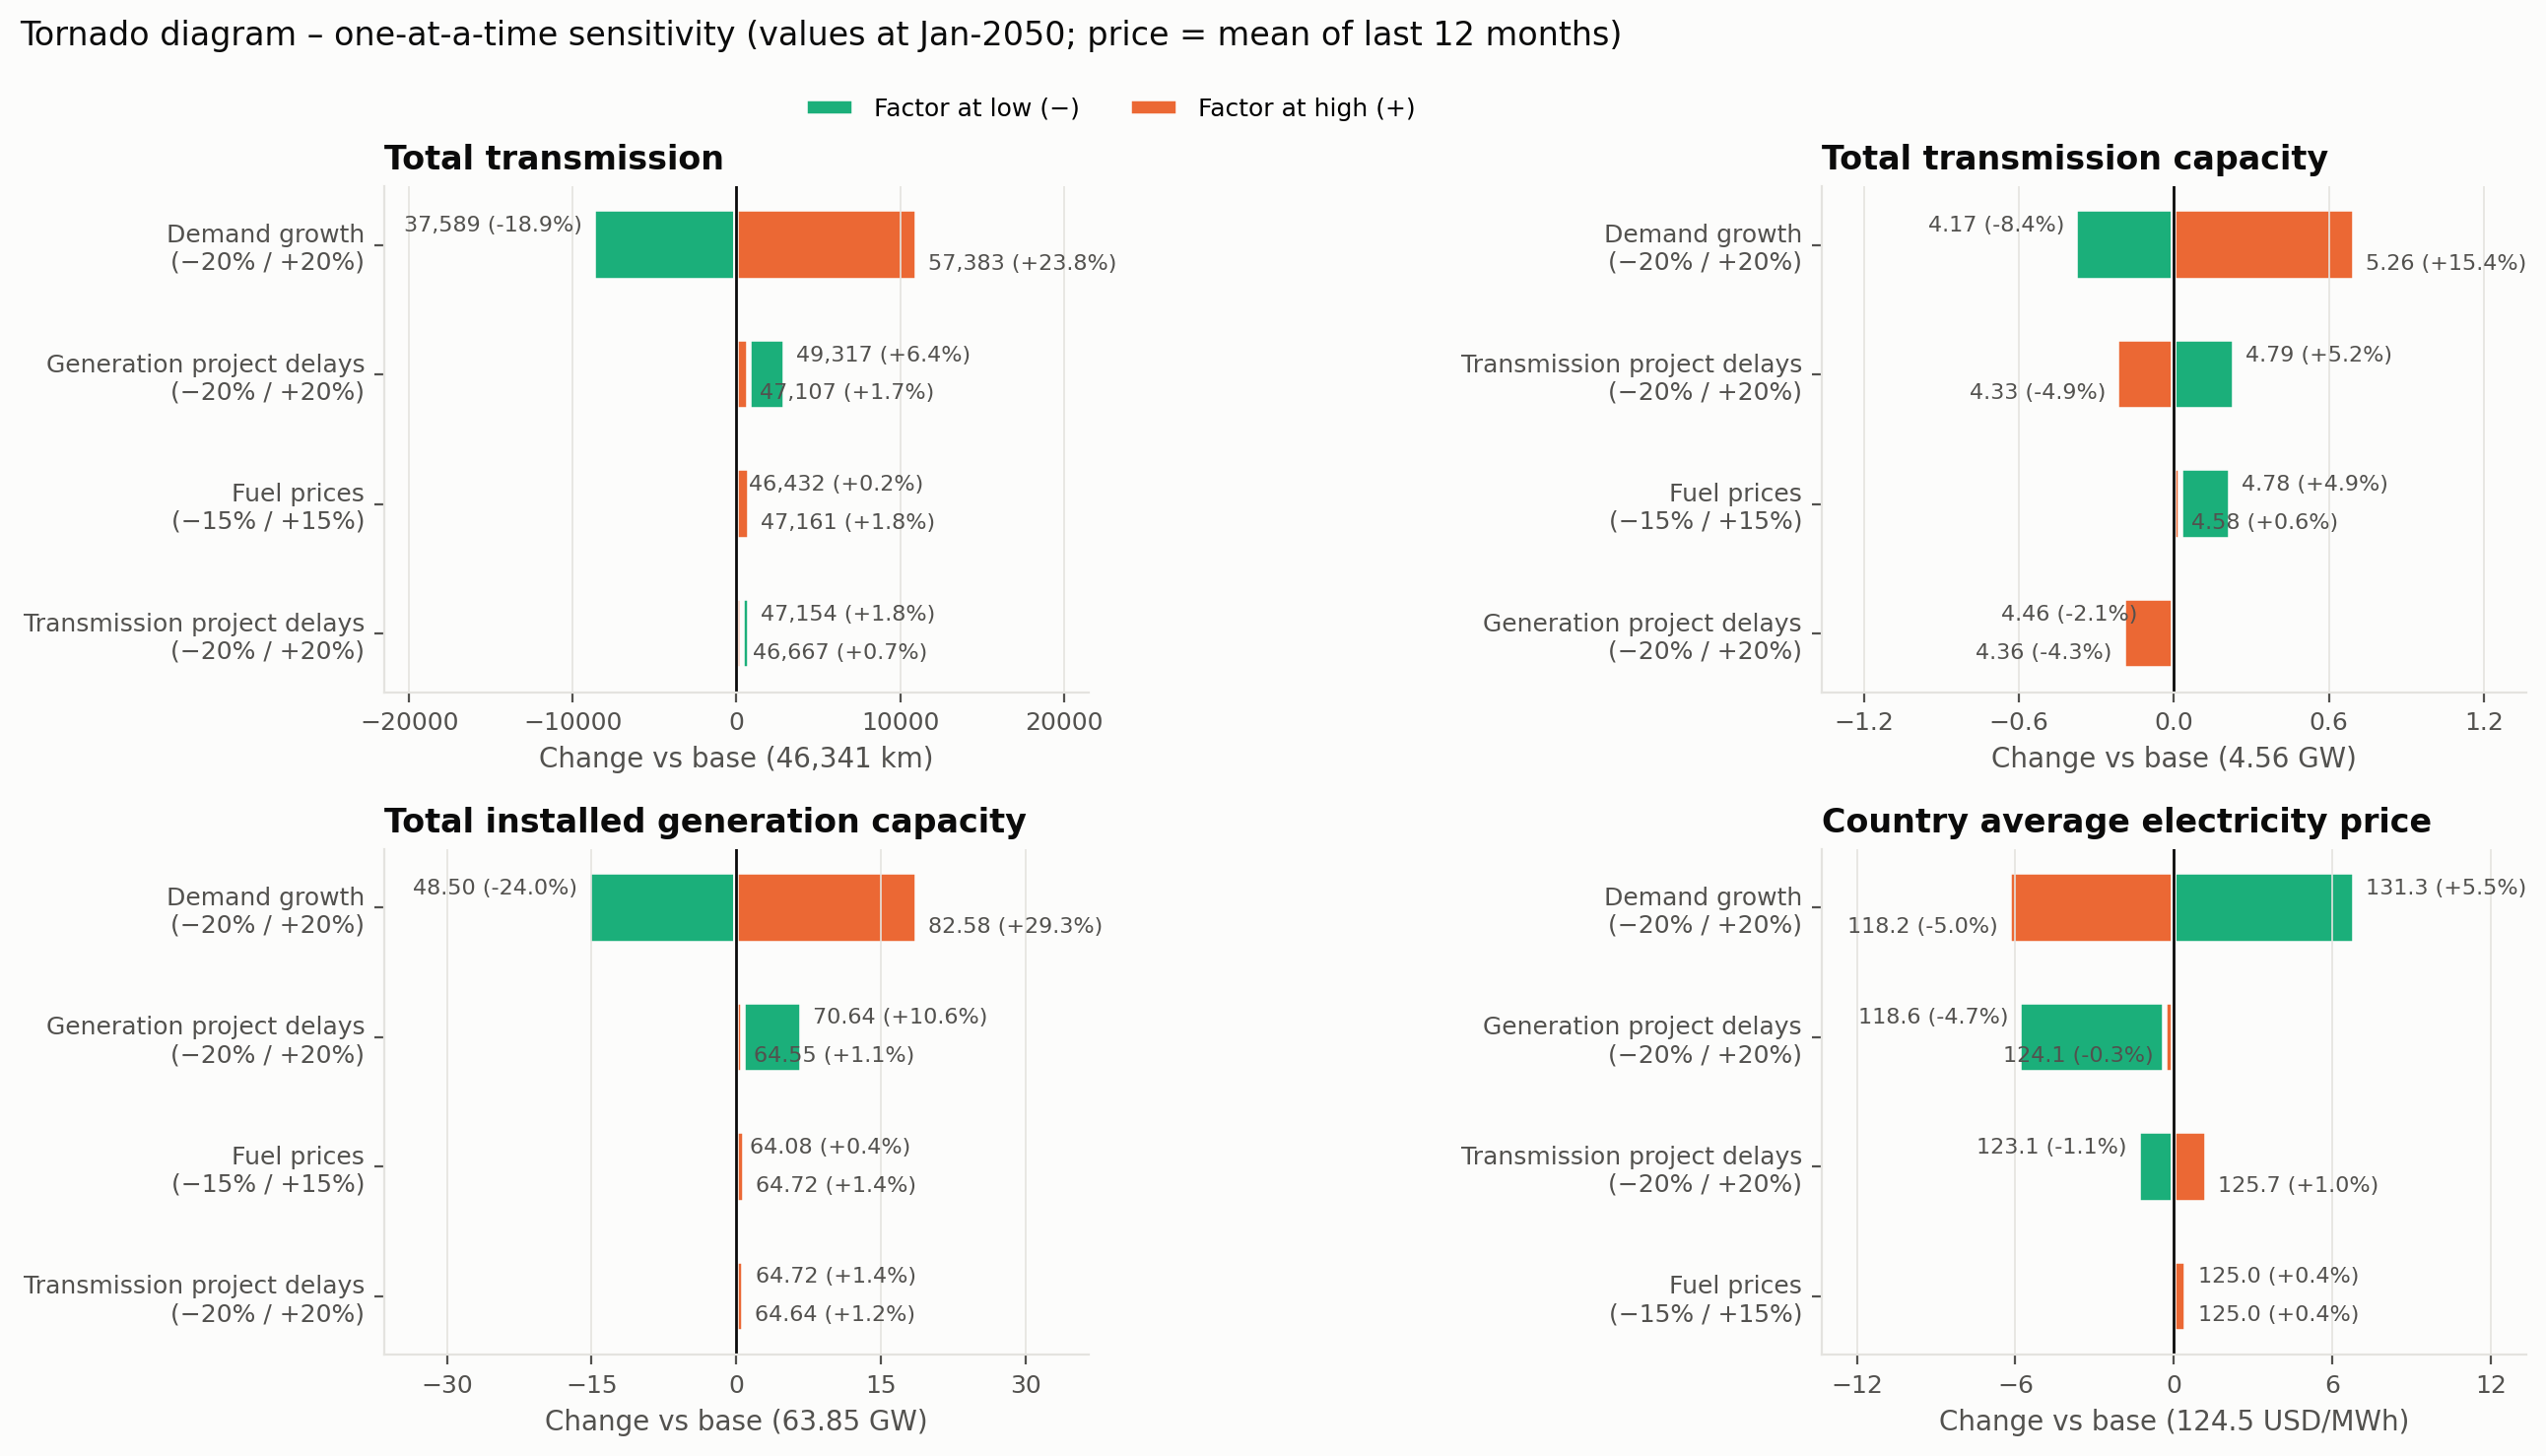
\includegraphics[width=\textwidth]{03_tornado.png}
  \caption{Tornado diagram. For each indicator, the bars show the change from the
  central case when one factor is set to the low and the high end of its range with
  the other three held at their reference value. Factors are ordered by swing,
  $|\text{high}-\text{low}|$. Values at January 2050; the price is the mean of the
  final twelve months.}
  \label{fig:tornado}
\end{figure*}

Table~\ref{tab:tornado} gives the numbers. A $\pm$20\,\% band on the 2050 demand level
moves required transmission from $-18.9$\,\% to $+23.8$\,\% and installed capacity from
$-24.0$\,\% to $+29.3$\,\%; the swing attributable to demand is nine times that of
generation lead times for transmission length. Fuel prices move the average price by
0.4\,\% in both directions --- not a sign error but a genuine non-monotonicity.

\begin{table}[tb]
  \centering
  \caption{One-at-a-time sensitivity. Change from the central case at January 2050
  with one factor at each end of its range. Factors ordered by swing within each
  indicator.}
  \label{tab:tornado}
  \scriptsize
  \begin{tabular}{@{}llrrr@{}}
    \toprule
    Indicator & Factor & Low & High & Swing \\
    \midrule
    \multirow{4}{*}{\shortstack[l]{Transmission\\ \si{\kilo\meter}, base \num{46341}}}
      & Demand growth        & $-18.9\%$ & $+23.8\%$ & \num{19794} \\
      & Generation lead time & $+6.4\%$  & $+1.7\%$  & \num{2210}  \\
      & Fuel price           & $+0.2\%$  & $+1.8\%$  & \num{729}   \\
      & Transmission lead time & $+1.8\%$ & $+0.7\%$ & \num{487}   \\
    \midrule
    \multirow{4}{*}{\shortstack[l]{Installed capacity\\ \si{\giga\watt}, base \num{63.85}}}
      & Demand growth        & $-24.0\%$ & $+29.3\%$ & \num{34.08} \\
      & Generation lead time & $+10.6\%$ & $+1.1\%$  & \num{6.09}  \\
      & Fuel price           & $+0.4\%$  & $+1.4\%$  & \num{0.64}  \\
      & Transmission lead time & $+1.4\%$ & $+1.2\%$ & \num{0.08}  \\
    \midrule
    \multirow{4}{*}{\shortstack[l]{Transfer capability\\ \si{\giga\watt}, base \num{4.56}}}
      & Demand growth        & $-8.4\%$  & $+15.4\%$ & \num{1.08}  \\
      & Transmission lead time & $+5.2\%$ & $-4.9\%$ & \num{0.46}  \\
      & Fuel price           & $+4.9\%$  & $+0.6\%$  & \num{0.19}  \\
      & Generation lead time & $-2.1\%$  & $-4.3\%$  & \num{0.10}  \\
    \midrule
    \multirow{4}{*}{\shortstack[l]{Average price\\ \si{\USD\per\mega\watt\hour}, base \num{124.5}}}
      & Demand growth        & $+5.5\%$  & $-5.0\%$  & \num{13.09} \\
      & Generation lead time & $-4.7\%$  & $-0.3\%$  & \num{5.52}  \\
      & Transmission lead time & $-1.1\%$ & $+1.0\%$ & \num{2.63}  \\
      & Fuel price           & $+0.4\%$  & $+0.4\%$  & \num{0.01}  \\
    \bottomrule
  \end{tabular}
\end{table}

The result is confirmed when all four factors move together
(Table~\ref{tab:spearman}): demand growth reaches $0.985$ for transmission length and
$0.973$ for installed capacity, close to the maximum a rank correlation can attain,
while no other factor exceeds $0.27$ in absolute value. The two methods agree, which is
the check that matters --- a one-at-a-time result surviving only in the absence of
interaction would not support the conclusion.

\begin{table}[tb]
  \centering
  \caption{Spearman rank correlation between each factor and each indicator over the
  120 Monte Carlo runs, in which all four factors vary simultaneously.}
  \label{tab:spearman}
  \small
  \begin{tabular}{@{}lrrrr@{}}
    \toprule
    Factor & Transmission & Transfer & Capacity & Price \\
           & [\si{\kilo\meter}] & [\si{\giga\watt}] & [\si{\giga\watt}] & [\si{\USD\per\mega\watt\hour}] \\
    \midrule
    Demand growth          & $\mathbf{0.985}$ & $\mathbf{0.835}$ & $\mathbf{0.973}$ & $\mathbf{-0.752}$ \\
    Transmission lead time & $0.112$  & $-0.142$ & $0.121$  & $-0.081$ \\
    Generation lead time   & $0.044$  & $0.081$  & $0.053$  & $-0.264$ \\
    Fuel price             & $-0.008$ & $-0.013$ & $-0.014$ & $-0.014$ \\
    \bottomrule
  \end{tabular}
\end{table}

\subsection{How wide the range of outcomes remains}
\label{sec:results:bands}

Figure~\ref{fig:bands} shows the P10--P90 envelope of each indicator. The envelopes are
narrow until the early 2030s and widen steadily thereafter --- the expected signature of
a system whose divergence is driven by a growth rate rather than a level.

\begin{figure*}[tb]
  \centering
  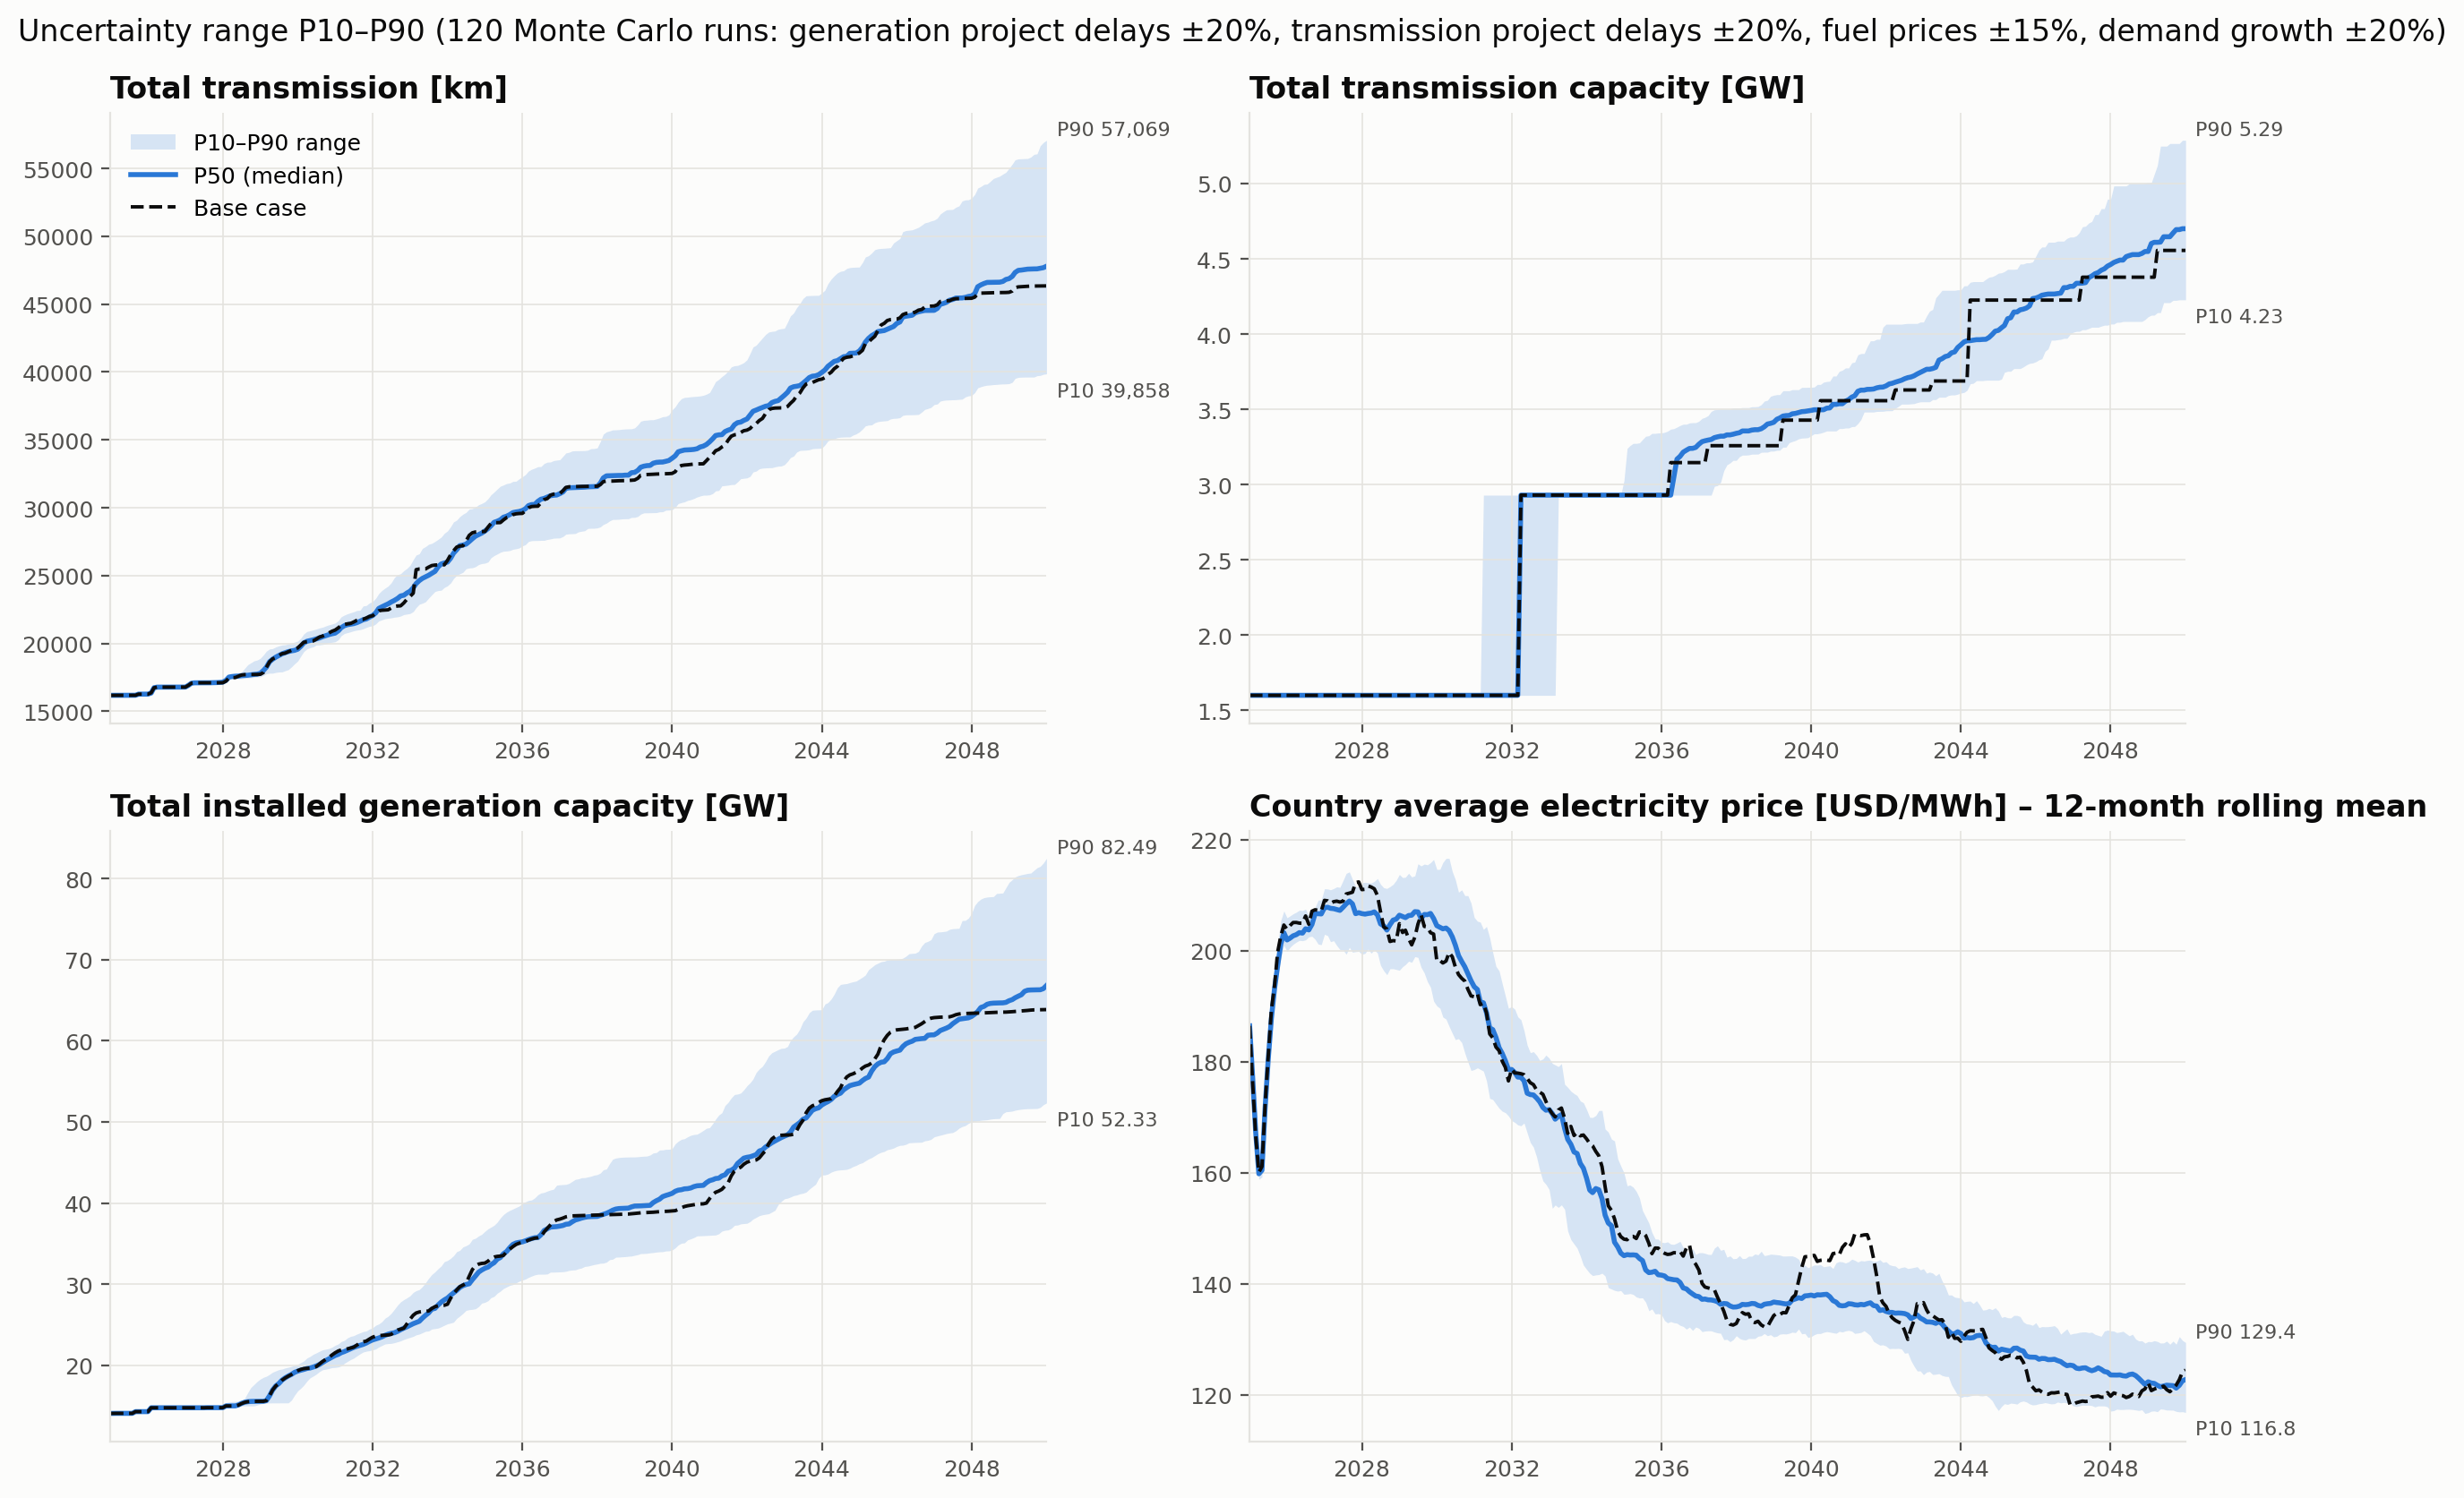
\includegraphics[width=\textwidth]{01_distribution_P10_P90_timeseries.png}
  \caption{P10--P90 envelope of the four indicators over 120 Monte Carlo runs, with
  the ensemble median and the central case. The band contains the central 80\,\% of
  outcomes.}
  \label{fig:bands}
\end{figure*}

By 2050 the ranges are substantial (Table~\ref{tab:bands}): installed capacity spans
\SIrange{52.3}{82.5}{\giga\watt} between the tenth and ninetieth percentile, a factor
of 1.6, and required transmission \SIrange{39858}{57069}{\kilo\meter}. The price range
is comparatively narrow, \SIrange{116.8}{129.4}{\USD\per\mega\watt\hour}. That
asymmetry is itself informative: what these uncertainties move is \emph{how much
infrastructure the country has to build}, far more than \emph{what electricity ends up
costing}.

\begin{table}[tb]
  \centering
  \caption{Indicator values at January 2050 over the 120 Monte Carlo runs.}
  \label{tab:bands}
  \small
  \begin{tabular}{@{}lrrrrr@{}}
    \toprule
    Indicator & Central & P10 & P50 & P90 & P90$-$P10 \\
    \midrule
    Transmission [\si{\kilo\meter}]            & \num{46341} & \num{39858} & \num{47788} & \num{57069} & \num{17211} \\
    Transfer capability [\si{\giga\watt}]      & \num{4.56}  & \num{4.23}  & \num{4.70}  & \num{5.29}  & \num{1.06}  \\
    Installed capacity [\si{\giga\watt}]       & \num{63.85} & \num{52.33} & \num{66.82} & \num{82.49} & \num{30.16} \\
    Average price [\si{\USD\per\mega\watt\hour}] & \num{124.5} & \num{116.8} & \num{122.8} & \num{129.4} & \num{12.59} \\
    \bottomrule
  \end{tabular}
\end{table}

The central case sits close to the median on transmission and capacity but at the
upper end of the price distribution. That is a consequence of the price
non-monotonicity identified in Table~\ref{tab:tornado}: because both an increase
and a decrease in several factors lower the price relative to the reference, the
reference is near a local maximum.

Supplementary Material~S4.2 reports the convergence of these
percentiles as runs are added. P10, P50 and P90 are stable from roughly 75 runs
onwards for every indicator, which is the evidence that 120 samples are sufficient
rather than an assumption that they are.

\subsection{Central, best and worst case}
\label{sec:results:extremes}

Table~\ref{tab:extremes} reports the three trajectories selected as described in
Section~\ref{sec:method:scenarios}. The best case on delivered price is run
\texttt{mc\_009}, in which demand grows 17.3\,\% faster than the reference; the
worst is \texttt{mc\_058}, in which it grows 16.5\,\% slower.

\begin{table}[tb]
  \centering
  \caption{Central, best and worst case. Best and worst are the Monte Carlo runs
  with the lowest and the highest country average price over the final twelve
  months. Percentages are relative to the central case.}
  \label{tab:extremes}
  \small
  \begin{tabular}{@{}lrrr@{}}
    \toprule
    & Central & Best (\texttt{mc\_009}) & Worst (\texttt{mc\_058}) \\
    \midrule
    \multicolumn{4}{@{}l}{\emph{Factor values}} \\
    Demand growth           & $0.0\%$ & $+17.3\%$ & $-16.5\%$ \\
    Generation lead time    & $0.0\%$ & $+9.8\%$  & $-5.4\%$  \\
    Transmission lead time  & $0.0\%$ & $+2.6\%$  & $+8.2\%$  \\
    Fuel price              & $0.0\%$ & $-2.5\%$  & $-1.1\%$  \\
    \midrule
    \multicolumn{4}{@{}l}{\emph{Indicators at January 2050}} \\
    Transmission [\si{\kilo\meter}]       & \num{46341} & \num{58562} $(+26.4\%)$ & \num{38927} $(-16.0\%)$ \\
    Transfer capability [\si{\giga\watt}] & \num{4.56}  & \num{5.03} $(+10.3\%)$  & \num{4.34} $(-4.8\%)$ \\
    Installed capacity [\si{\giga\watt}]  & \num{63.85} & \num{86.40} $(+35.3\%)$ & \num{49.18} $(-23.0\%)$ \\
    Average price [\si{\USD\per\mega\watt\hour}] & \num{124.5} & \num{114.9} $(-7.6\%)$ & \num{135.6} $(+9.0\%)$ \\
    \bottomrule
  \end{tabular}
\end{table}

This is the central empirical finding, and it runs against the intuition that higher
demand means a more stressed and therefore more expensive system. The mechanism is
visible in the technology mix (Figures~\ref{fig:captech} and~\ref{fig:gentech}): in
the best case onshore wind reaches \SI{52.05}{\giga\watt} against
\SI{34.83}{\giga\watt} centrally and \SI{25.47}{\giga\watt} in the worst, and solar PV
\SI{11.51}{\giga\watt} against \SI{8.33} and \SI{5.24}{\giga\watt}. Faster demand
growth sustains a price signal long enough for low-cost renewable capacity to clear the
profitability threshold earlier and in greater volume, and once in place that capacity
depresses the marginal price. Slow demand growth suppresses the investment signal and
leaves the system leaning on thermal plant --- \SI{10.2}{\tera\watt\hour\per\year} in
the worst case against \SI{5.6}{\tera\watt\hour\per\year} in the best --- ending with a
higher average price despite a smaller system.

\begin{figure*}[tb]
  \centering
  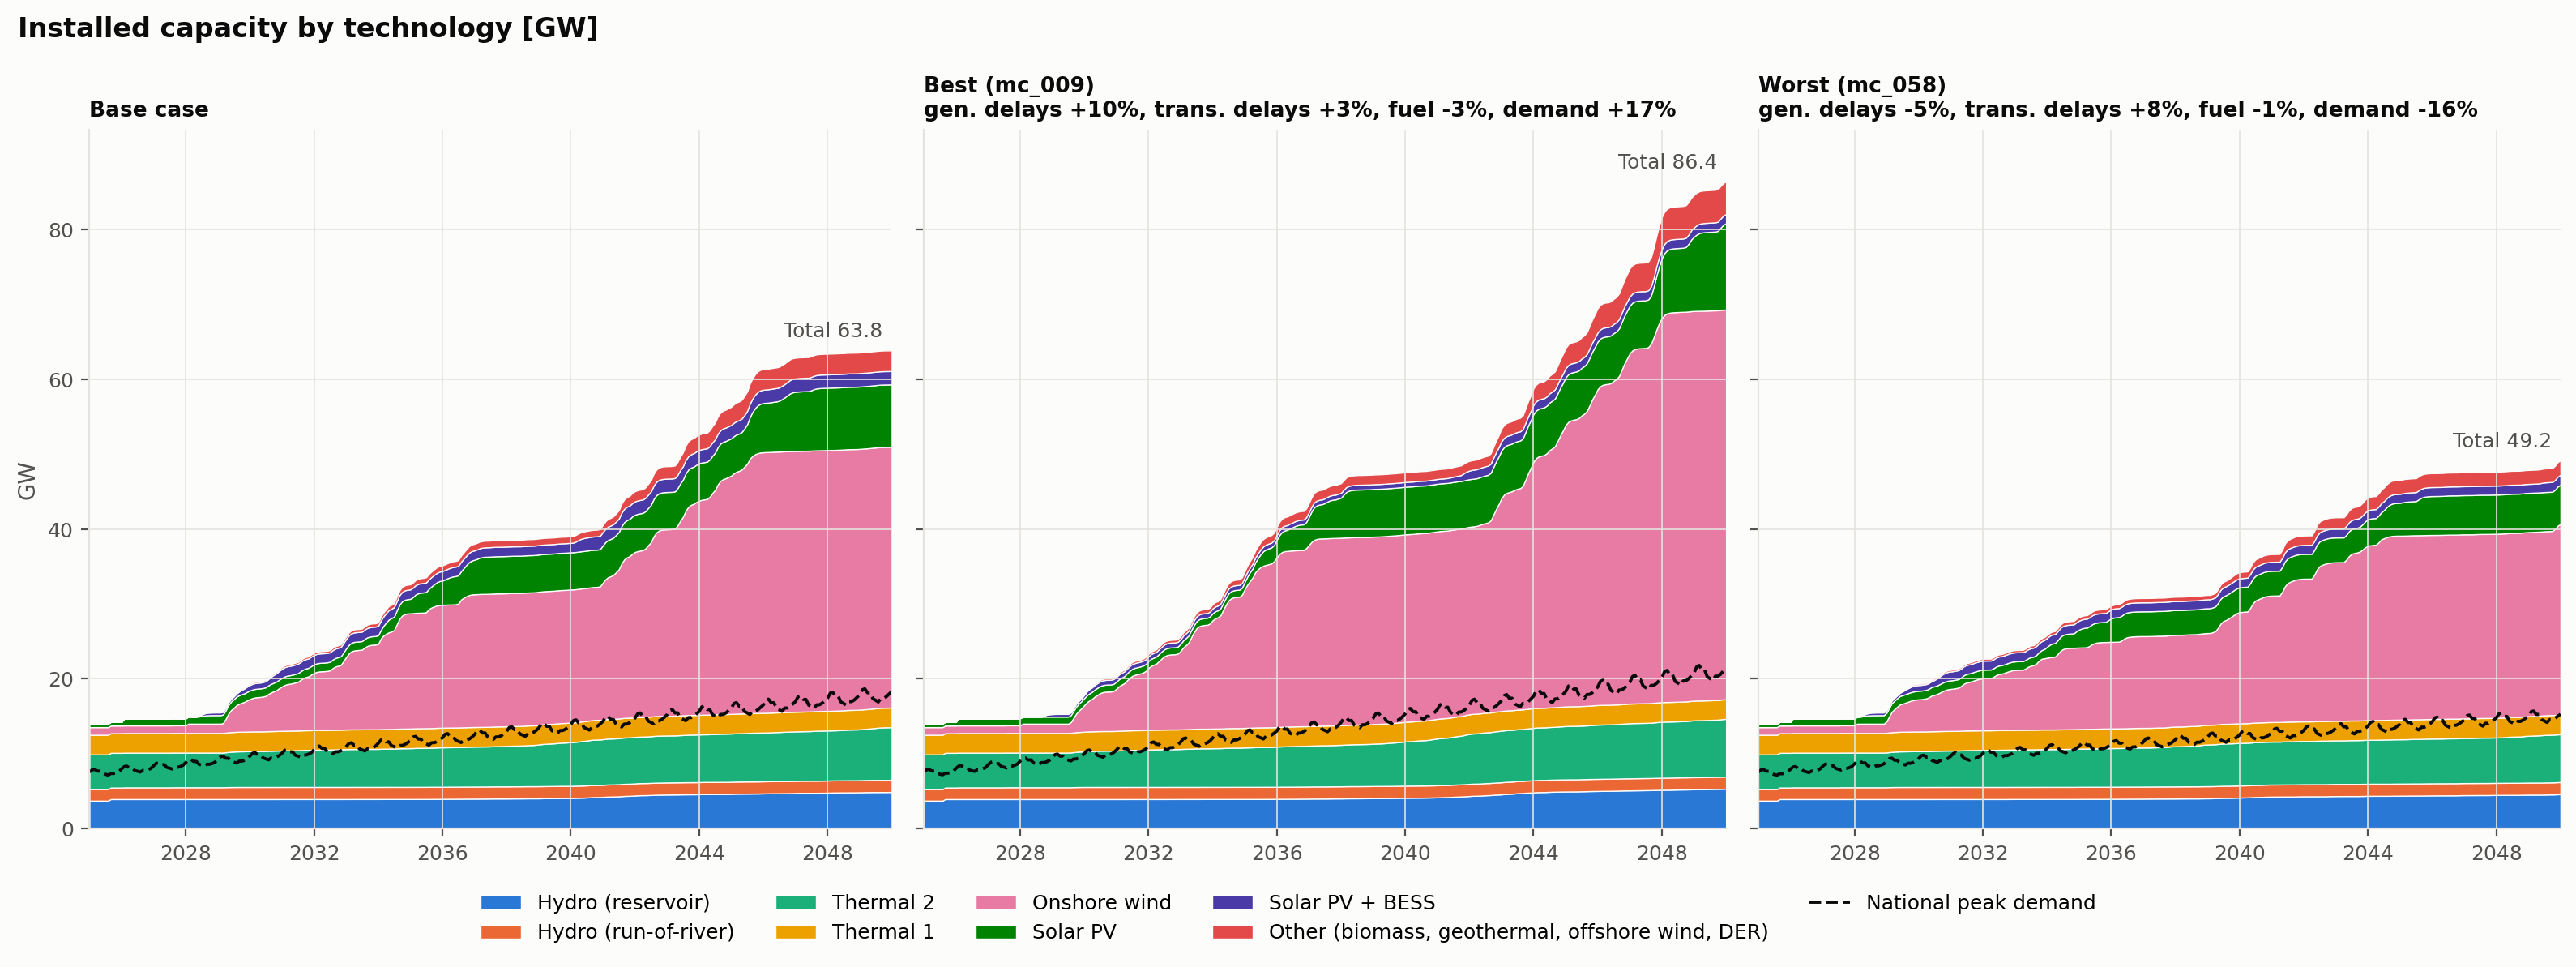
\includegraphics[width=\textwidth]{05_installed_capacity_by_technology.png}
  \caption{Installed capacity by technology for the central, best and worst case.
  The dashed line is national peak demand. Fourteen model technologies are
  aggregated into eight series; the mapping is given in Supplementary
  Material~S5.3.}
  \label{fig:captech}
\end{figure*}

\begin{figure*}[tb]
  \centering
  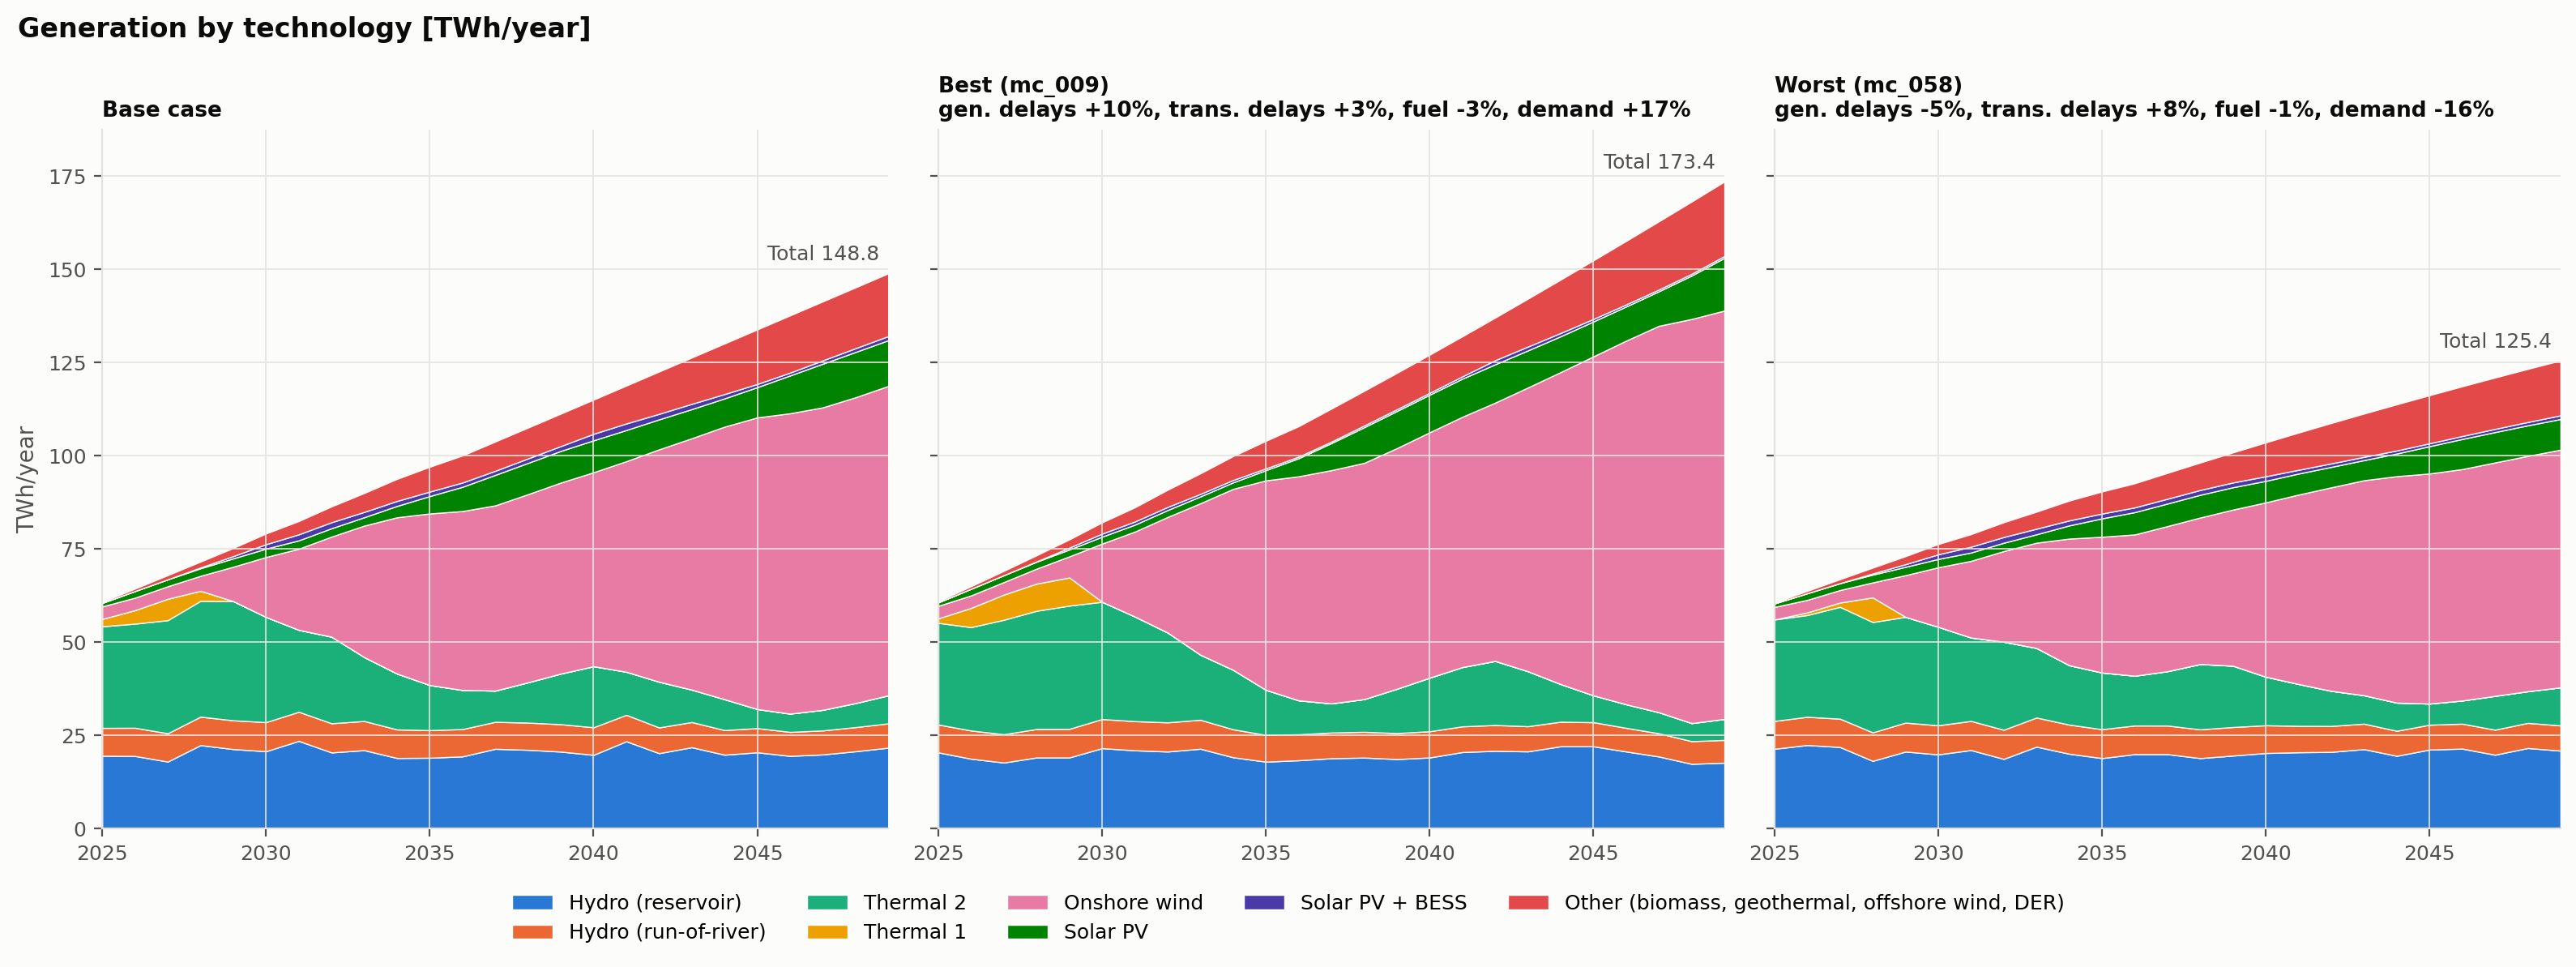
\includegraphics[width=\textwidth]{06_generation_by_technology.png}
  \caption{Annual generation by technology for the central, best and worst case.}
  \label{fig:gentech}
\end{figure*}

The corollary is uncomfortable for a planner. The least-cost trajectory is also the
most infrastructure-intensive: the best case requires \SI{58562}{\kilo\meter} of
network, 26.4\,\% more than the central case and 50\,\% more than the worst case,
together with 10.3\,\% more inter-zonal transfer capability. The cheapest electricity
in this system is not obtained by building less; it is obtained by building more,
faster. Figure~\ref{fig:price} shows the resulting price paths and
Figure~\ref{fig:transmission} the transmission requirement.

\begin{figure*}[tb]
  \centering
  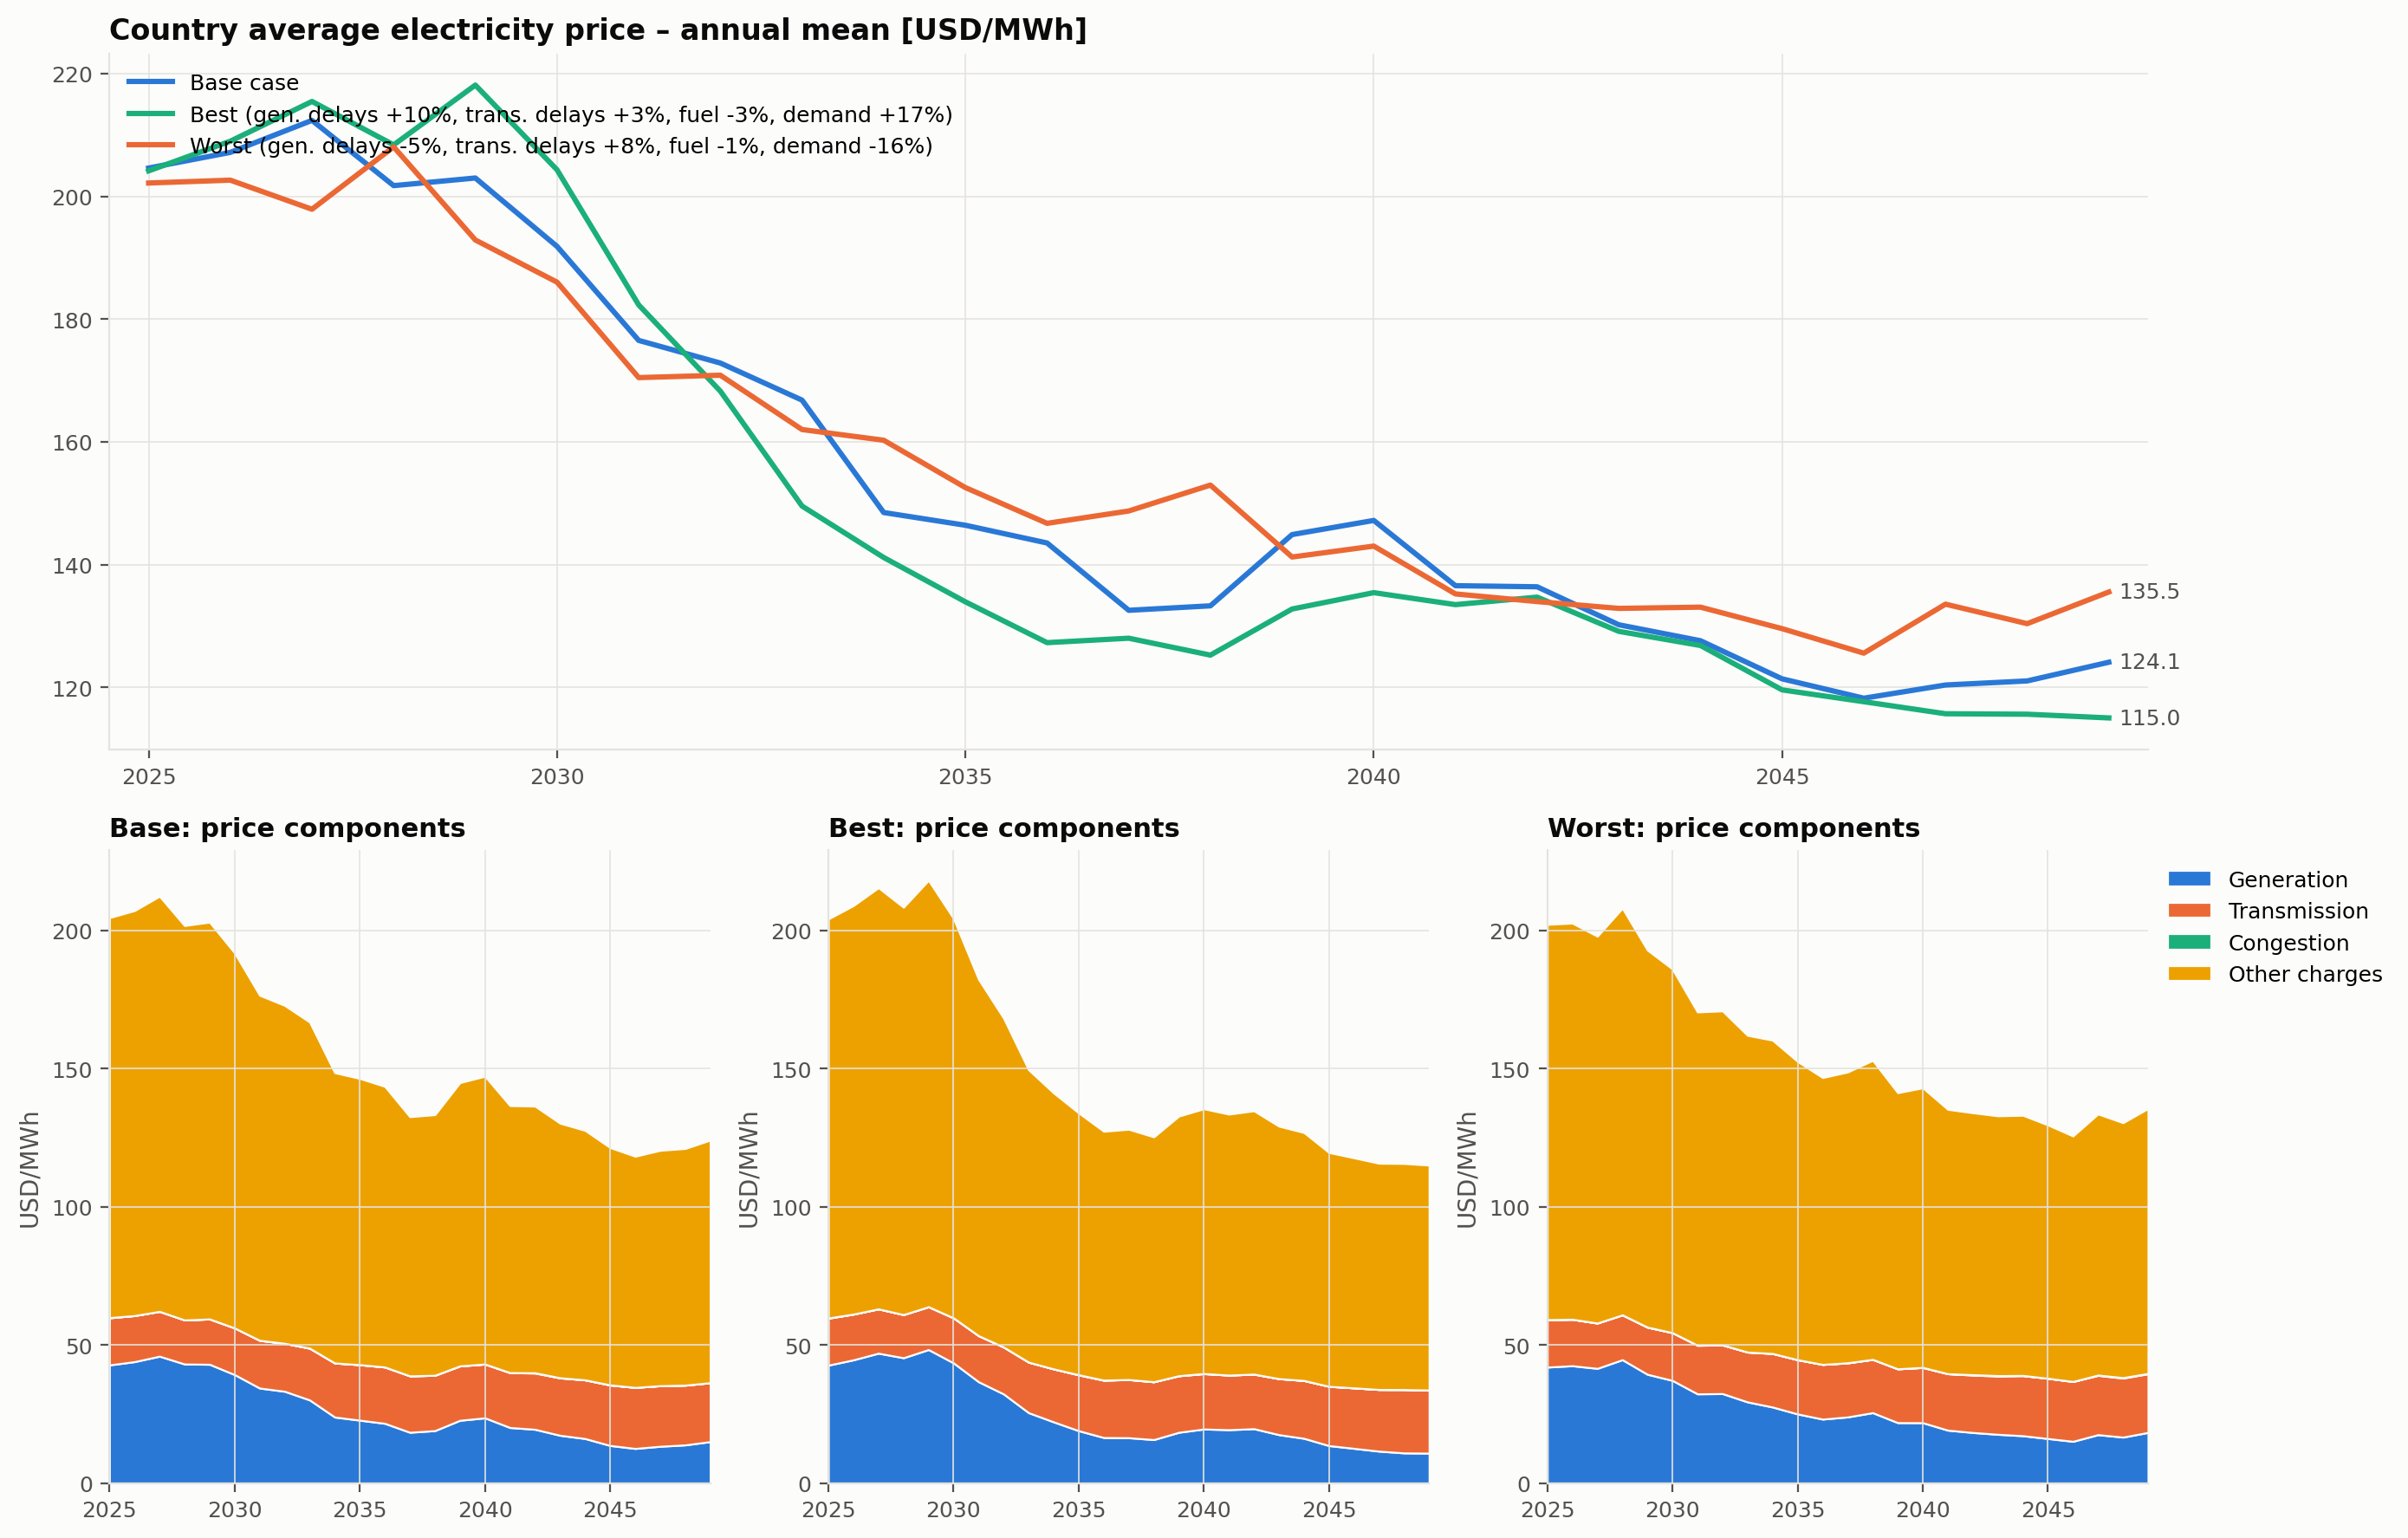
\includegraphics[width=\textwidth]{04_price_best_worst.png}
  \caption{Country average electricity price for the central, best and worst case.}
  \label{fig:price}
\end{figure*}

\begin{figure*}[tb]
  \centering
  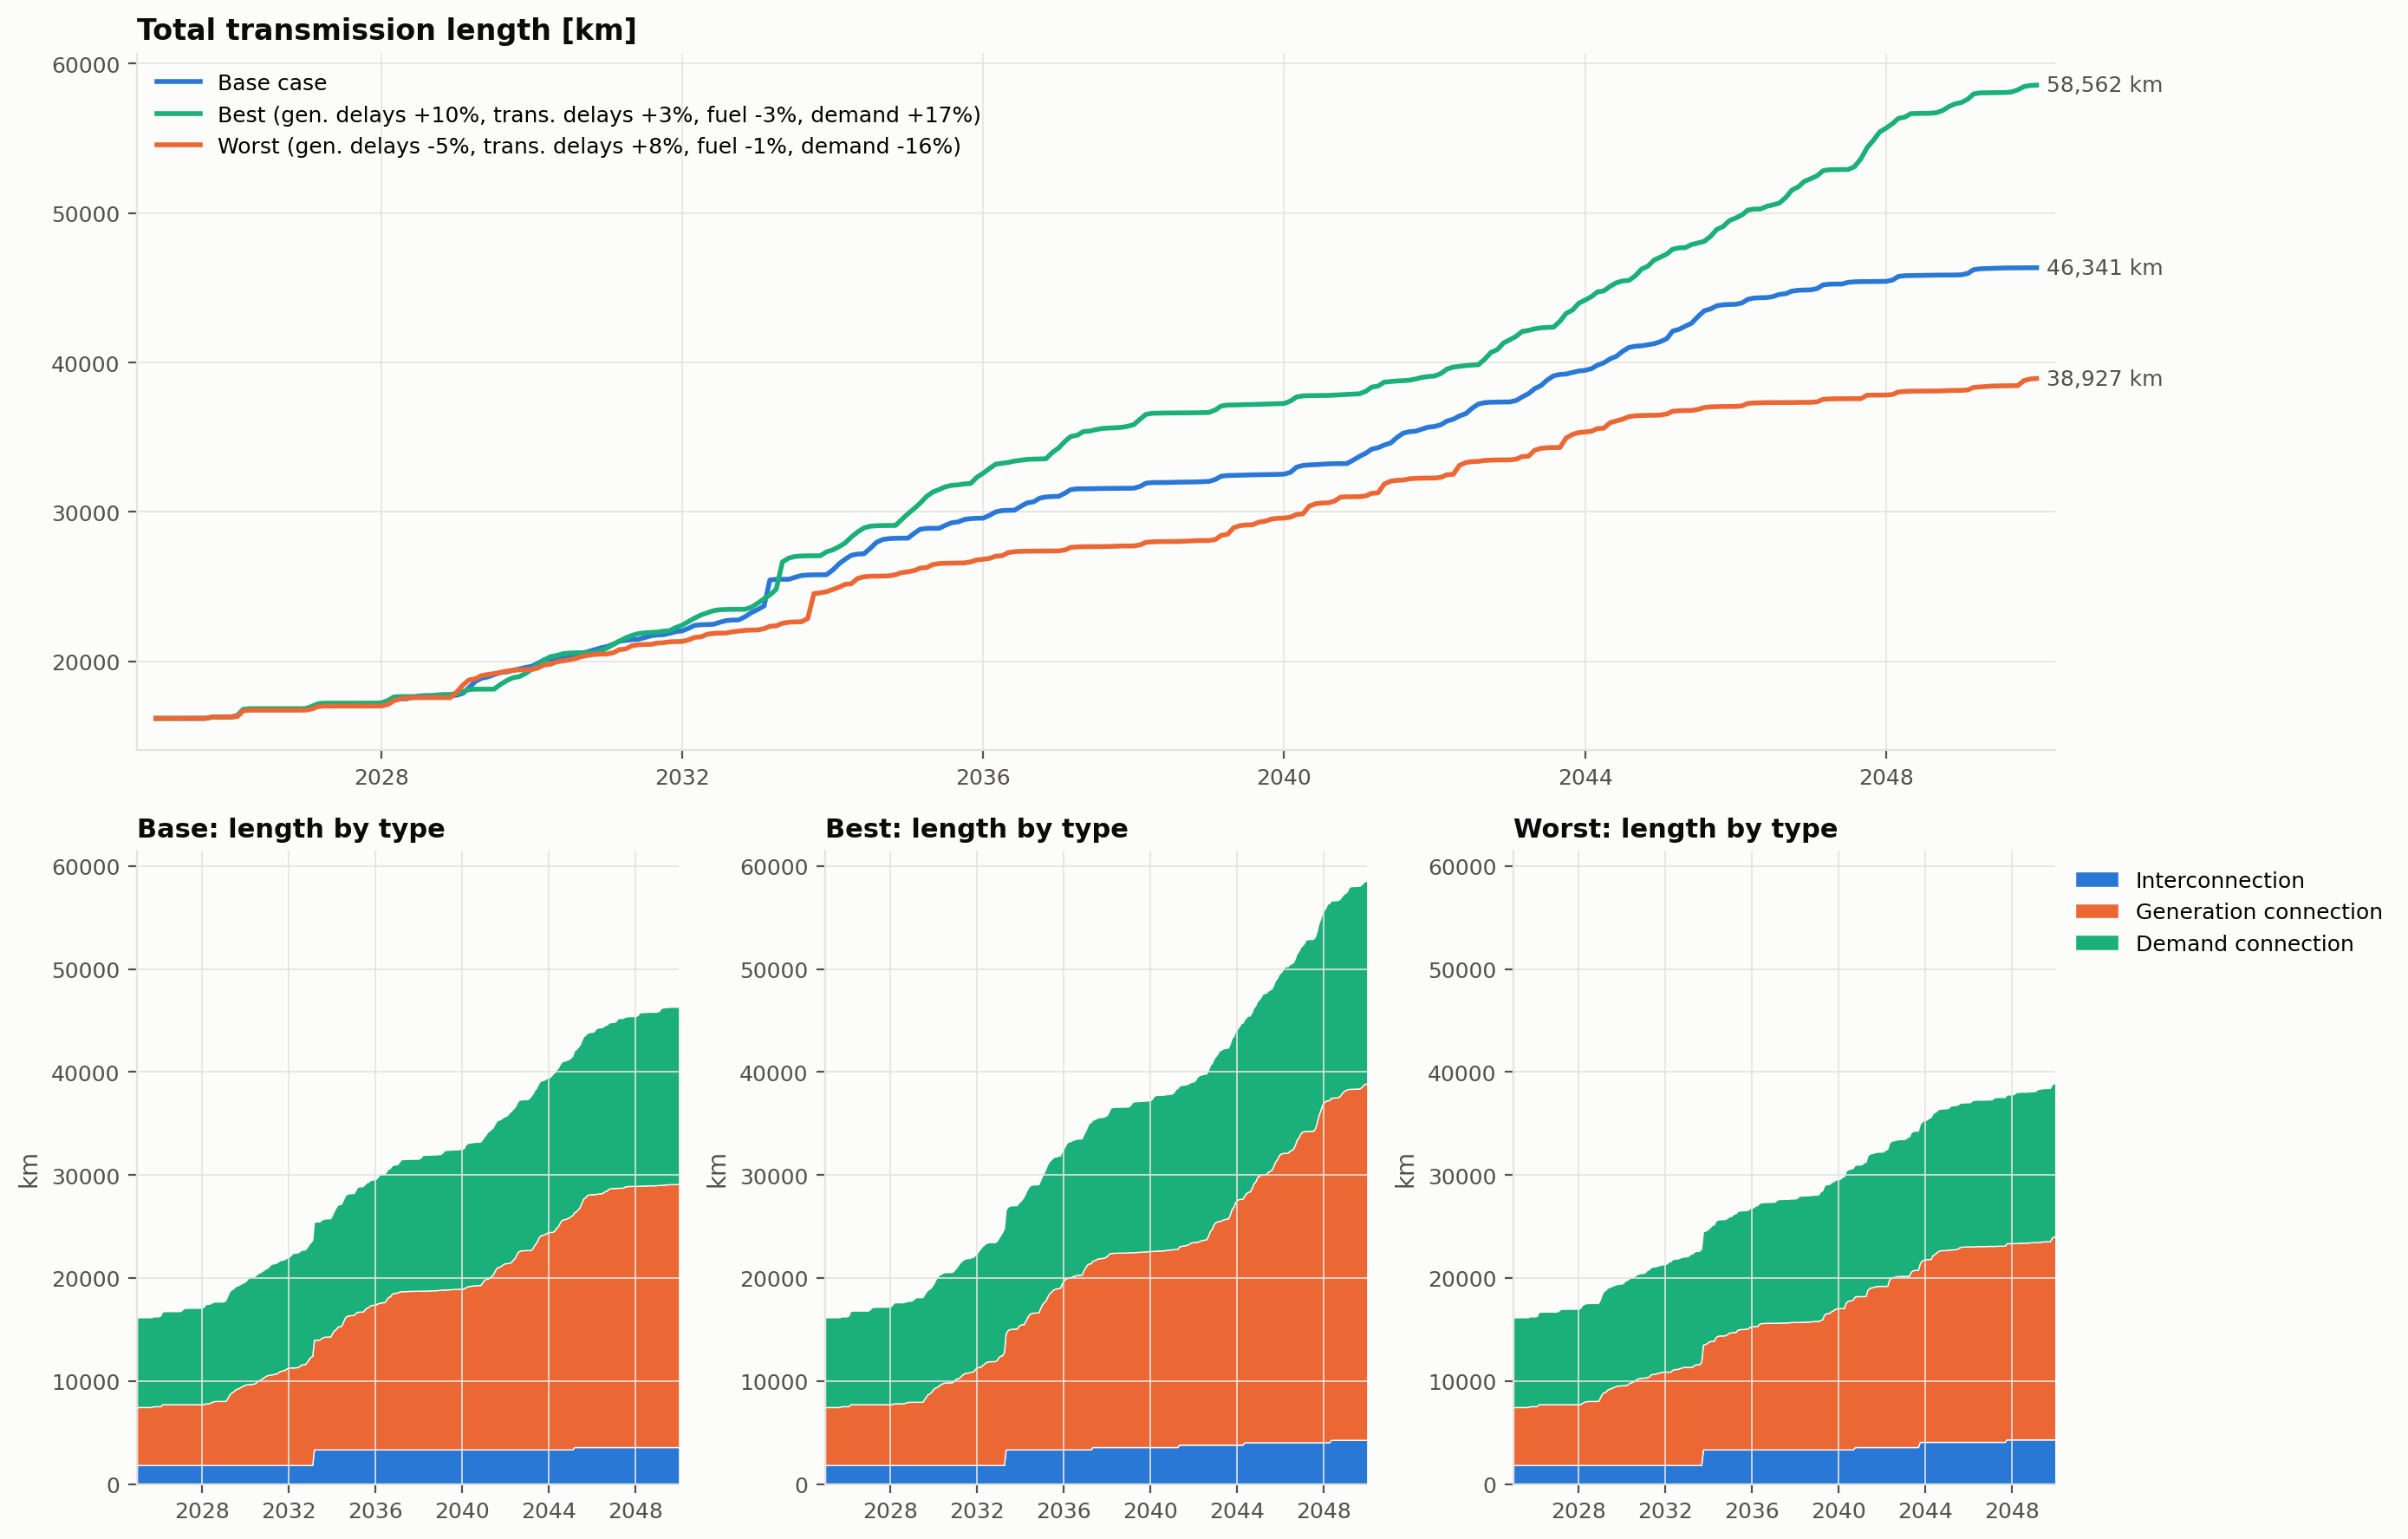
\includegraphics[width=\textwidth]{08_transmission_km.png}
  \caption{Transmission network by category --- demand connection, generation
  connection and interconnection --- for the central, best and worst case.}
  \label{fig:transmission}
\end{figure*}

A second observation concerns the delay factors. The best case has \emph{longer}
generation lead times than the central case ($+9.8$\,\%) and the worst case has
shorter ones ($-5.4$\,\%). This is not evidence that delays are beneficial; it is a
consequence of their weakness relative to demand. Within the sampled ranges, the
demand draw determines the outcome and the delay draw is close to noise, so the
extreme runs on price carry essentially arbitrary delay values. Reporting this
explicitly is more honest than selecting extreme runs that happen to tell a tidier
story, and it is itself the clearest statement of the ranking: in this system, over
these ranges, lead times do not decide the outcome.

\subsection{Where the uncertainty acts}
\label{sec:results:where}

Decomposing transmission by category (Figure~\ref{fig:transmission}) locates the
effect. Network built for demand connection scales directly with peak demand and
inherits the demand factor's variance in full; network built to connect generation
follows the investment decision and inherits it indirectly. Inter-zonal corridor
capability is the least sensitive of the three and the only one where transmission
lead time ranks second rather than fourth (Table~\ref{tab:tornado}): a longer pipeline
defers reinforcements, which the series topology converts into persistent congestion
rather than a different final capacity. That is why transmission lead time barely
registers in the aggregate indicators while remaining operationally important --- the
model builds much the same network in the end, and what the lead time changes is
\emph{when} it is available.

\section{Discussion}
\label{sec:discussion}

\subsection{Why transmission matters for Peru's energy transition}

The results give the grid a specific and quantified role. Between 2025 and 2050 the
central case requires the transmission network to grow from \SI{16180}{\kilo\meter}
to \SI{46341}{\kilo\meter} --- a factor of 2.9 --- and the plausible range extends
to \SI{57069}{\kilo\meter} at the ninetieth percentile. That requirement is not
driven by a decarbonisation target; the model has none. It is driven by the
locational mismatch described in Section~\ref{sec:peru:zones}: the capacity that the
profitability rule selects is wind and solar, and those resources sit away from the
centre zone that holds 60\,\% of demand.

This is the point at which Peru's longitudinal topology stops being a descriptive
detail. In a meshed system, a corridor constraint has alternatives; in a system
where the south reaches the rest of the country only through the centre, it does
not. \citet{herrera2019} show for northeast Brazil that transmission constraints
bound wind expansion directly, and \citet{ritter2019} show for Europe that delayed
interconnection changes the final generation mix rather than merely postponing it.
Our results are consistent with both, with the qualification that in Peru the
binding quantity is the \emph{rate} at which network can be delivered relative to
the rate at which demand grows.

\subsection{Demand growth as the governing uncertainty}

That demand dominates is, in retrospect, structurally explicable. Demand enters the
model at the root of every chain: it sets the adequacy trigger, it sets the residual
demand that the dispatch clears and hence the price signal that drives the
profitability trigger, and it sets the zonal peaks that drive demand-connection
network directly. Fuel prices, by contrast, enter only at the dispatch, and in a
system that ends up 85\,\% non-thermal in capacity terms, a cost shift on the
shrinking thermal margin has little leverage. The rank correlation of $-0.014$ for
fuel prices on the average price is not a modelling artefact; it is what one should
expect once the marginal technology is no longer the one burning the fuel.

The policy reading is uncomfortable, because demand growth is the one driver on the
list that planning does not control and forecasting handles poorly. It is also the
driver for which the model's own range ($\pm$20\,\% on the 2050 level) is arguably
conservative for an emerging economy with incomplete electrification and potential
industrial loads. Methods for long-horizon demand uncertainty
\citep{lee2022,alvarez2026} are therefore not a peripheral refinement for Peruvian
planning but the main lever on the quality of the answer.

\subsection{The price result and what it does not say}

The finding that faster demand growth lowers the long-run average price requires
careful statement, because it is easy to over-read.

It is a statement about a \emph{long-run average} under an investment rule that
responds to profitability. Faster demand sustains the price signal long enough for
low-cost renewable capacity to clear the threshold earlier and in greater volume;
that capacity then depresses the marginal price. It is not a statement that demand
growth is costless --- the same runs require 26\,\% more transmission and 35\,\%
more generation capacity, and the model prices neither the capital at risk nor the
land and social cost of that build-out. Nor is it a statement about short-run
prices: Figure~\ref{fig:price} shows the high-demand case \emph{above} the others
through the late 2020s, before the capacity it induces arrives.

Three structural caveats bound it further. The model has no endogenous retirement,
so thermal plant persists and the mix shifts by addition rather than by replacement.
Storage and grid-enhancing technologies are disabled at the switch level in every
run reported here, so the substitution between flexibility and network documented by
\citet{sousa2024} and \citet{sadeghian2026} is absent; enabling them would plausibly
reduce the transmission requirement of the high-demand case and weaken exactly the
corollary we emphasise. And the dispatch uses one representative day per month,
which under-represents sustained scarcity.

\subsection{Infrastructure delays and long-term reliability}

Lead times rank second and third in our design, well behind demand. We do not read
this as evidence that delays are unimportant for Peru, and the distinction matters.

What the result says is that, over a $\pm$20\,\% band around current practice,
lead times do not change the \emph{size} of the system that gets built by 2050. What
it does not say is that they do not change the system's condition along the way.
Section~\ref{sec:results:where} shows the mechanism: longer transmission pipelines
defer reinforcements, and in a series topology the deferral surfaces as congestion
between zones rather than as a different terminal capacity. An indicator measured at
January 2050 is poorly suited to capture that, and this is a limitation of our
reporting choice as much as a property of the system. A study aimed specifically at
reliability would need congestion-hours, curtailment and unserved energy as
indicators rather than terminal stocks.

There is also a range effect. We varied lead times by $\pm$20\,\% around the
Peruvian base case, which is a plausible band for incremental administrative
improvement. It is not the band relevant to institutional failure: the literature on
delay causes --- right-of-way disputes, licensing, local opposition
\citep{sun2026,boateng2026} --- describes multi-year slippage on individual projects,
well outside $\pm$20\,\% of a planned stage. Our ranking is conditional on the
ranges in Table~\ref{tab:factors}, as any sensitivity ranking must be.

\subsection{Thermal dependence and fuel-price exposure}

Peru's gas dependence is the feature most often identified as its principal
vulnerability \citep{rudnick2019,enerdata2024,colinacalvo2024}, and our results
qualify that view in a specific way. Fuel prices are the weakest of the four drivers
on every indicator, with a swing of \SI{0.005}{\USD\per\mega\watt\hour} on the 2050
average price --- effectively zero.

The qualification is temporal, not substantive. The model's own trajectory removes
the exposure: by 2050 thermal plant supplies \SI{7.5}{\tera\watt\hour\per\year} of
\SI{148.8}{\tera\watt\hour\per\year} in the central case. Fuel-price risk is
therefore a near-term exposure that the expansion path itself retires, provided the
expansion path is delivered. If it is not --- if the network cannot be built at the
rate the investment rule assumes --- the system remains thermal for longer and the
exposure persists. Read that way, fuel-price risk in Peru is better understood as a
\emph{consequence} of transmission delivery than as an independent risk to be hedged
separately, which is a different policy prescription from the one usually drawn.

\subsection{Renewable integration and transmission coordination}

The central case reaches 84.9\,\% non-thermal capacity by 2050 with no renewable
target, driven by profitability alone. That is a stronger statement about the
competitiveness of Peruvian wind and solar than a target-constrained model could
make, and it aligns with the optimisation-based findings of \citet{fiestas2024} and
\citet{delacruz2024} from a different methodological direction --- which is worth
noting, since agreement between an optimising and a behavioural model on the
direction of the transition is more informative than either alone.

Where the two diverge is on what it costs to get there. An optimisation model
coordinates generation siting and network expansion by construction; our model does
not, because the Peruvian institutional arrangement does not. Transmission for
generation is triggered by \emph{confirmed} projects rather than anticipated ones
(Section~\ref{sec:method:trans}), which is reactive by design, and transmission lead
times exceed generation lead times. \citet{herding2024} quantify the prize for
closing that gap --- around 10\,\% lower total investment and up to 30\,\% less
network expansion under coordination --- and \citet{sauma2006} formalise the
proactive-versus-reactive distinction that underlies it. Our results indicate that
Peru is firmly on the reactive side, and that the cost of remaining there rises with
demand growth.

Complementary options would attack the same constraint from the demand side.
Distributed generation reduces the inter-zonal transfers a longitudinal grid must
support \citep{antoniolli2022,wu2025,sheng2026}, and grid-enhancing technologies
raise the capability of existing corridors without new right-of-way
\citep{sadeghian2026}. Both are represented in the model but disabled in this
experiment; quantifying them for Peru is the obvious next study, and our results
indicate where the gain would be largest --- the Z2--Z3 corridor under high demand.

\subsection{Policy implications}

Four implications follow, stated in the order our evidence supports them.

\emph{Transmission delivery capacity is the planning variable to protect.} Demand
growth governs the outcome and is outside the planner's control; what the planner
controls is whether the network can keep pace. Since the least-cost outcome is also
the most network-intensive, the risk is asymmetric: under-building the grid forecloses
the cheap trajectory.

\emph{Anticipatory network planning has a measurable value here.} The reactive
trigger plus the lead-time asymmetry is a structural bottleneck, not a parameter
choice. Moving the trigger from confirmed to anticipated projects is a regulatory
decision with a quantifiable payoff \citep{sauma2006,herding2024}.

\emph{Demand forecasting deserves the modelling effort that fuel-price hedging
currently receives.} Given a 1:900 ratio in rank correlation between demand and fuel
prices for transmission requirements, the allocation of analytical attention in
Peruvian planning is not proportionate to the sensitivities.

\emph{Restoring a predictable procurement signal matters more than the price it
clears.} The profitability trigger in the model responds to a sustained price
signal. The suspension of the auction mechanism \citep{campodonico2022,torres2026}
removes exactly that, and \citet{delrio2026} show that in Latin America the cost of
capital rather than resource quality determines what is financed --- a channel our
model represents only through the discount rate.

\subsection{Comparison with other Latin American systems}

Peru's three-zone series topology is unusual in the region and it drives the result.
Brazil's meshed system gives alternatives when a corridor binds, and the constraint
appears as regional heterogeneity in deployment efficiency \citep{dasilva2025} or as
curtailment \citep{herrera2019}, rather than as a single critical path. Chile's
system is also longitudinal and its curtailment problem is well documented; the
comparison with Peru is therefore the more instructive one, and \citet{reyes2025}
note that Chile has moved considerably further from a comparable liberalised base.

The common regional thread is institutional. \citet{guliev2022} and
\citet{sempertegui2017} identify regulatory sovereignty rather than engineering as
the barrier to Andean interconnection, and \citet{boateng2026} show institutional
quality conditioning the response to otherwise identical incentives. Our finding
that lead times matter less than demand should not be generalised to systems with
weaker institutions or wider delay distributions than the $\pm$20\,\% band we
sampled.

\subsection{Methodological implications}

Two points generalise beyond Peru.

First, pairing a system dynamics model with a designed experiment changes what the
model can claim. A small set of named scenarios shows what a model does; it cannot
separate a structural result from an artefact of one input assumption. Here the
designed experiment turned a plausible narrative --- that a gas-dependent system
faces fuel-price risk --- into a measured ranking that contradicts it. The cost is
modest: 129 runs, mechanisable, with the design fixed before execution.

Second, reporting both one-at-a-time and all-factors-varying evidence is worth the
redundancy. The two answer different questions and have complementary weaknesses,
and their agreement (Tables~\ref{tab:tornado} and~\ref{tab:spearman}) is what makes
the ranking defensible. Where they disagreed we would have to report it, and that
disagreement would itself be a finding about interaction.

We would add a third, more practical observation. The infrastructure of this study
--- resumable execution, a design fixed and archived before any simulation ran, and
explicit checks that each run actually produced data --- was not incidental. Several
of those checks caught silent failures during execution that would otherwise have
entered the results as missing data rather than as errors. For simulation
experiments of this size, that machinery deserves to be part of the method rather
than left to each author's practice.

\section{Conclusions and policy implications}
\label{sec:conclusions}

We set out to establish which uncertainty governs the trajectory of the Peruvian
power system, rather than to forecast that trajectory. A system dynamics model with
explicit generation and transmission pipelines, coupled to a congestion-aware
dispatch and subjected to a 129-run designed experiment over 2025--2050, gives an
unambiguous answer.

\paragraph{Demand growth dominates, by an order of magnitude.} Over the sampled
ranges, demand growth reaches Spearman rank correlations of $0.985$ with required
transmission, $0.973$ with installed capacity and $-0.752$ with the average price,
while no other factor exceeds $0.27$ in absolute value. A $\pm$20\,\% band on the
2050 demand level moves required transmission by $-18.9$\,\% to $+23.8$\,\% and
installed capacity by $-24.0$\,\% to $+29.3$\,\%. The one-at-a-time and the
all-factors-varying evidence agree on this ranking.

\paragraph{Fuel-price risk is weaker than the literature on Peru implies, and for a
structural reason.} Fuel prices are the weakest driver on three of four indicators,
moving the 2050 average price by \SI{0.005}{\USD\per\mega\watt\hour}. The model's own
expansion path removes the exposure: thermal generation falls to
\SI{7.5}{\tera\watt\hour\per\year} of \SI{148.8}{\tera\watt\hour\per\year} by 2050.
Fuel-price risk in Peru is therefore better understood as a near-term exposure
contingent on transmission delivery than as an independent long-run risk.

\paragraph{The least-cost trajectory is the most network-intensive.} Faster demand
growth lowers the long-run average price, because it sustains the price signal long
enough to pull forward low-cost wind and solar. The best case on delivered price
requires \SI{58562}{\kilo\meter} of transmission, 26.4\,\% more than the central case
and 50\,\% more than the worst, with 10.3\,\% more inter-zonal transfer capability.
For a system whose grid is already the binding constraint, the cheap path is the one
that demands most of the planner.

\paragraph{Lead times change when, not how much.} Transmission lead times rank last
or second-to-last on terminal indicators, but the decomposition by transmission
category shows why: the model builds much the same network either way, and the
deferral surfaces as inter-zonal congestion rather than as a different system size.
Terminal stocks are the wrong indicator for that effect, which is a limitation of
our reporting and a clear direction for the next study.

\paragraph{The expansion is renewable without being told to be.} The central case
reaches 84.9\,\% non-thermal capacity by 2050 under a profitability rule alone, with
no target, mandate or carbon price. That a behavioural model and the
optimisation-based Peruvian literature \citep{fiestas2024,delacruz2024} agree on the
direction of the transition, having disagreed on almost everything methodological, is
itself worth recording.

\subsection*{Policy implications}

The practical reading is that Peruvian planning attention is not proportionate to
the sensitivities. Effort devoted to fuel-price exposure buys little; effort devoted
to (i) long-horizon demand forecasting, (ii) the institutional capacity to deliver
transmission at the rate demand requires, and (iii) moving the network trigger from
confirmed to anticipated generation projects \citep{sauma2006,herding2024}, buys a
great deal. Restoring a predictable procurement signal matters for the same reason:
the investment response in the model is to a sustained price signal, and the
suspension of the auction mechanism removes it.

\subsection*{Limitations}

The ranking is conditional on the ranges in Table~\ref{tab:factors}; a wider delay
distribution, such as the multi-year slippage documented for individual projects
elsewhere, could change it. Storage and grid-enhancing technologies are disabled in
every run reported here, so the substitution between flexibility and network is
absent and the transmission requirement of the high-demand case is, if anything,
overstated. Retirements are exogenous, the dispatch uses one representative day per
month, and the distributions are uniform ranges of admissibility rather than
estimated densities. Each of these is documented with its consequence in the
supplementary material.

\subsection*{Further work}

Three extensions follow directly. First, enabling storage and grid-enhancing
technologies and re-running the same design would quantify how much network the
flexibility options actually displace --- our results identify the Z2--Z3 corridor
under high demand as where the gain would be largest. Second, replacing terminal
stocks with congestion-hours, curtailment and unserved energy as reported indicators
would capture the timing effect of lead times that our indicators miss. Third, the
same design applied to Brazil and Chile with the same model structure would separate
what is Peruvian from what is a property of longitudinal systems generally; the
model and driver used here are already structured for that comparison.


\section*{Data and code availability}
The Vensim model, the complete input workbook, the experimental design, the
simulation driver, the post-processing code and the commented notebook that
regenerates every figure in this paper are openly available at
\url{https://github.com/sebastianzapatar/peru-expansion-uncertainty}.
\todo{Replace with the DOI of the archived release before submission.}
Nothing required to reproduce the results is available only on request.

\section*{Declaration of competing interest}
The authors declare that they have no known competing financial interests or
personal relationships that could have appeared to influence the work reported in
this paper.

\section*{Acknowledgements}
\todo{Funding and acknowledgements to be completed by the team.}

\bibliographystyle{elsarticle-harv}
\bibliography{refs}

\end{document}
